\documentclass[10pt,a4paper]{article}

\usepackage[margin=2.5cm]{geometry}
\usepackage[T1]{fontenc}
\usepackage{lmodern}
\usepackage{amsmath,amssymb}
\usepackage{booktabs}
\usepackage{graphicx}
\usepackage{subcaption}
\usepackage{xcolor}
\usepackage[colorlinks=true,linkcolor=blue!50!black,urlcolor=blue!50!black]{hyperref}

% Highlighted placeholder for things still to write or verify
\usepackage{todonotes}

\title{\textbf{Image Dithering: Notes}}
\author{Xavier Doni}
\date{\today}

\begin{document}
\maketitle
\tableofcontents
\newpage

% ------------------------------------------------------------------
\section{What is Dithering?}
\label{sec:what}
\subsection{Quantisation}

A digital image stores each pixel as a value from a limited set of
intensities. In the real world, light is continuous, and the human eye can perceive millions of colours.
Whereas a display (or file format) can only represent a \emph{reduced} palette of colors,
every pixel must be mapped to one of the available values. This is known as \emph{quantisation}.

\begin{figure}[htbp]
  \centering
  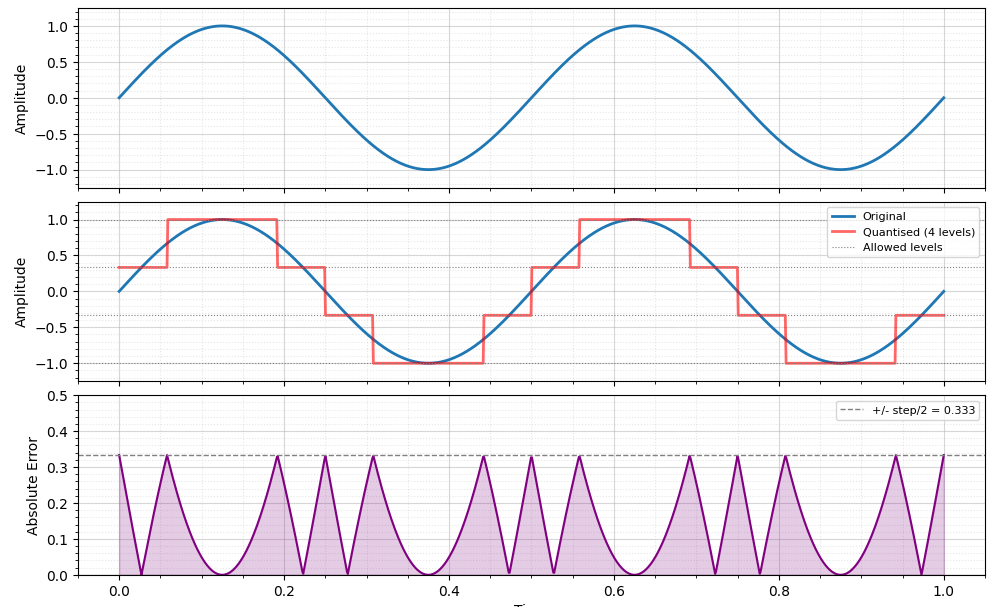
\includegraphics[width=0.9\textwidth]{../output/Section_1/Figure_1_1.png}
  \caption{Quantisation of a continuous wave. The original signal (blue) quantised to 2 bits = 4 levels (red).}
  \label{fig:quant-example}
\end{figure}


If we look at images, let a single channel of an image be a function $I(x,y)\in[0,255]$.
A quantiser with $L$ levels snaps each value to the nearest of $L$ evenly
spaced values:
\begin{equation}
  \Delta = \frac{255}{L-1}, \qquad
  q(v) = \Delta \cdot \operatorname{round}\!\left(\frac{v}{\Delta}\right).
\end{equation}
The difference between an input value and its quantized value is called the \emph{quantisation error},
denoted by $e = v - q(v)$, and always satisfies $|e|\le \Delta/2$. For a colour image the quantiser is applied to
the red, green and blue channels independently, giving $L^3$ possible colours
(Table~\ref{tab:levels}).

\begin{table}[htbp]
  \centering
  \caption{Palette size as a function of levels per channel $L$.}
  \label{tab:levels}
  \begin{tabular}{rrrr}
    \toprule
    $L$ & Grayscale shades & Colours ($L^3$) & Step $\Delta$ \\
    \midrule
    2   & 2   & 8          & 255   \\
    3   & 3   & 27         & 127.5 \\
    4   & 4   & 64         & 85    \\
    6   & 6   & 216        & 51    \\
    256 & 256 & 16,777,216 & 1     \\
    \bottomrule
  \end{tabular}
\end{table}

As $L$ increase, the quantisation error decreases hence the amount of information lost decreases.
However, the number of colours grows cubically with $L$,
so any small increase in $L$ can drastically increase a file size.
This is why many image formats use a small palette of colours, and why dithering is important.

\newpage

\subsection{Dithering}

\emph{Dithering} is the family of techniques that arranges the available values spatially
so that, viewed from a distance, the eye averages neighbouring pixels
and perceives intermediate tones that the palette cannot represent directly.
In short, dithering trades spatial resolution for tonal resolution.
Instead of mapping each pixel independently to the nearest palette colour, dithering
\emph{remembers} the quantisation error and distributes it to neighbouring pixels, such that
the average tone is preserved.

\begin{figure}[htbp]
  \centering
  \begin{subfigure}{0.40\textwidth}
    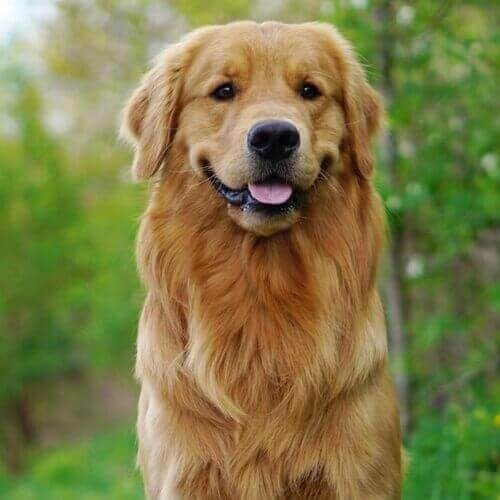
\includegraphics[width=\linewidth]{../data/images/Golden-Retriever.jpeg}
    \caption{Original}
  \end{subfigure}
  \begin{subfigure}{0.40\textwidth}
    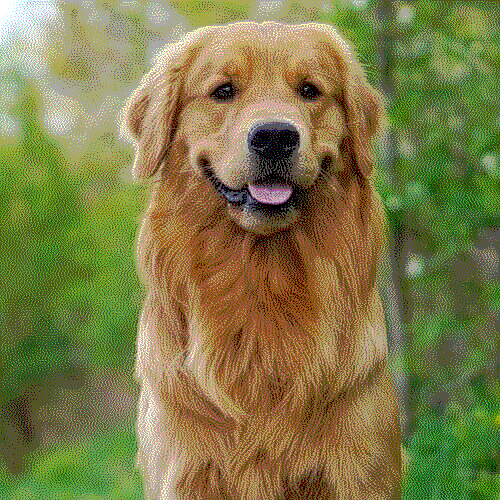
\includegraphics[width=\linewidth]{../output/Section_1/Figure_1_2.png}
    \caption{Dithered}
  \end{subfigure}
  \caption{Original versus dithered}
\end{figure}

Dither is routinely used in processing of both digital audio and visual data,
and is a key technique in computer graphics.
The result is almost always a more faithful reproduction of the original image.
We'll focus on the visual case, where dithering is used to reduce the number of colours in an image.

\begin{figure}[htbp]
  \centering
  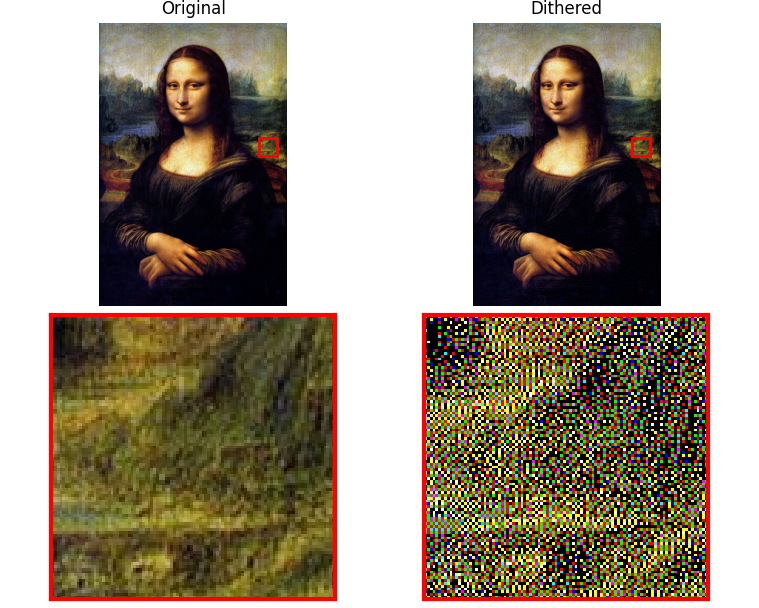
\includegraphics[width=0.70\textwidth]{../output/Section_1/Figure_1_3.png}
  \caption{Dithering of the Mona Lisa. The original image (left)
  is quantised to 2 levels per channel and then dithered (right).}
  \label{fig:dither-example}
\end{figure}

\newpage

% ------------------------------------------------------------------
\section{Historical Context}
\label{sec:history}

Early display hardware could show only a handful of colours at once.
The IBM Colour Graphics Adapter (CGA), introduced in 1981 with the IBM PC, is the classic example.
This was the first monitors in the market to display color.
Image resolution was low, and the palette was limited to 16 colours.
Its 16-colour palette is built from four on/off signals:
red, green, blue and an intensity bit (RGBI). Sixteen colours need only
four bits per pixel, since $2^4 = 16$.

\begin{figure}[htbp]
  \centering
  \begin{subfigure}{0.58\textwidth}
    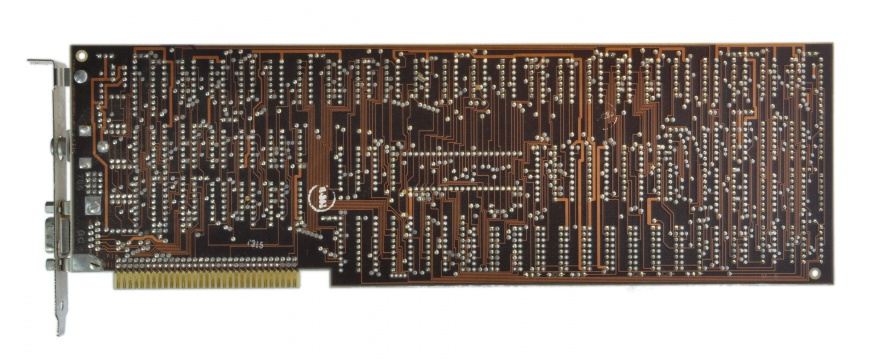
\includegraphics[width=\linewidth]{../data/figures/IBM-Color-Graphics-Adapter.jpg}
    \caption{IBM CGA card}
  \end{subfigure}
  \begin{subfigure}{0.36\textwidth}
    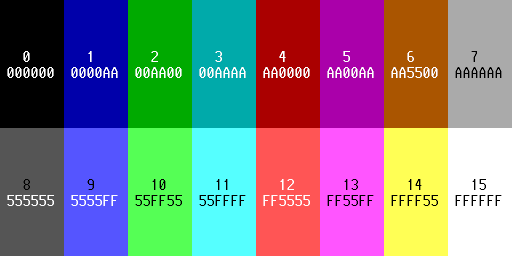
\includegraphics[width=\linewidth]{../data/figures/IBM-5153-Color.png}
    \caption{16 colour palette on a CGA monitor}
  \end{subfigure}
  \caption{The IBM Colour Graphics Adapter (CGA) and its 16-colour palette.}
\end{figure}

This should not be confused with ``16-bit colour'' (High Color) used in modern systems,
which uses 16 bits per pixel and yields $2^{16} = 65{,}536$ colours
(Table~\ref{tab:bits}).

\begin{table}[htbp]
  \centering
  \caption{Bits per pixel versus number of distinct colours.}
  \label{tab:bits}
  \begin{tabular}{lrr}
    \toprule
    Name & Bits per pixel & Colours \\
    \midrule
    CGA palette          & 4  & 16         \\
    ``16-bit'' High Color & 16 & 65,536     \\
    24-bit True Color    & 24 & 16,777,216 \\
    \bottomrule
  \end{tabular}
\end{table}



CGA offered several video modes, each with a different resolution and palette size
suited to different applications with different memory constraints:
\begin{itemize}
  \item a 160x100 mode with 16 colours
  \item a 320x200 mode with 4 colours
  \item a 640x200 mode with 2 colours
\end{itemize}

Each mode was a compromise between resolution and colour depth.
For some programs, they were small enough to make use of the 16-colour mode.
But the limited palette for programs with a larger resolution was a problem.
Programmers therefore mixed pixel patterns to imitate the missing colours,
which is a major reason dithering became widespread.
In the 1980s, dithering was used in many games and graphics programs to
simulate more colours than the hardware could display.

\smallskip   % \smallskip \medskip \bigskip

Take a look at Figure \ref{fig:cga-examples}.
The three images are from the same era, but they use different CGA modes.
For example, the game \ref{fig:pakupaku}, the original Pac-Man, uses the 160x100 16 colour mode.
The game makes use of the full palette, each ghost is a different colour, each fruit is a different colour,
and the yellow Pac-Man really pops out of the screen. However, although in this mode the resolution
is limited, the user is still able to experience the game just fine and play it without any problems.
While the program \ref{fig:pcpaint} uses the 320x200 4 colour mode, PCPaint is designed
to create images, and the user is able to select the colours they want to use.
At that the time, the 4 colour mode was a compromise between resolution and colour depth.
% \smallskip \medskip \bigskip
Finally, \ref{fig:simcity} uses the 640x200 monochrome mode.
It's a city-building simulation game where the user is able to build their own city.
It's a very complex game, to display all the information on the screen, the program uses the 640x200 monochrome mode.
However, beause of the limited palette, the program uses dithering to simulate gray tones
and a non-square pixel ratio that deforms the fonts.
The use of dithering helps to make up for the lack of colours and makes the game more visually appealing.

%PakuPaku in 160x100 16 color mode
%PCPaint in 320 × 200 3rd palette low intensity, showing a typical low-resolution interface.
%Note the use of dithering to overcome the CGA palette limitations.
%SimCity in 640 × 200 monochrome.
%Note the use of dithering to simulate gray tones and a non-square pixel ratio that deforms the fonts.

\newpage

\begin{figure}[htbp]
  \centering
  \begin{subfigure}{0.40\textwidth}
    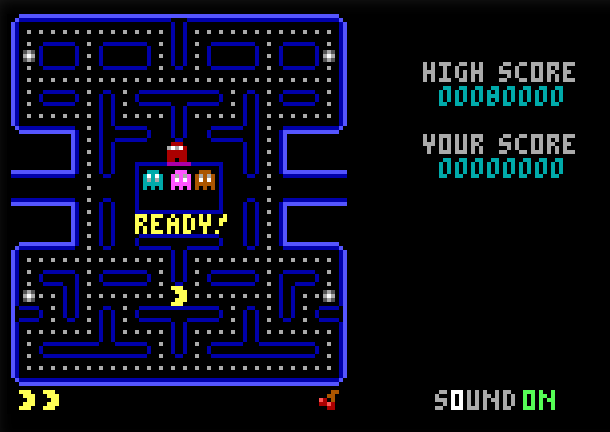
\includegraphics[width=\linewidth]{../data/figures/Paku-Paku.png}
    \caption{PakuPaku in 160x100 16 color mode}
    \label{fig:pakupaku}
  \end{subfigure}
  \begin{subfigure}{0.45\textwidth}
    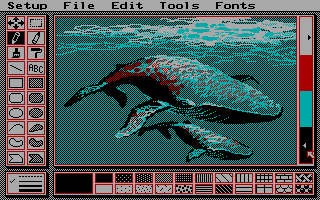
\includegraphics[width=\linewidth]{../data/figures/PC-Paint.png}
    \caption{PCPaint in 320×200 3rd palette low intensity}
    \label{fig:pcpaint}
  \end{subfigure}
  \begin{subfigure}{0.60\textwidth}
    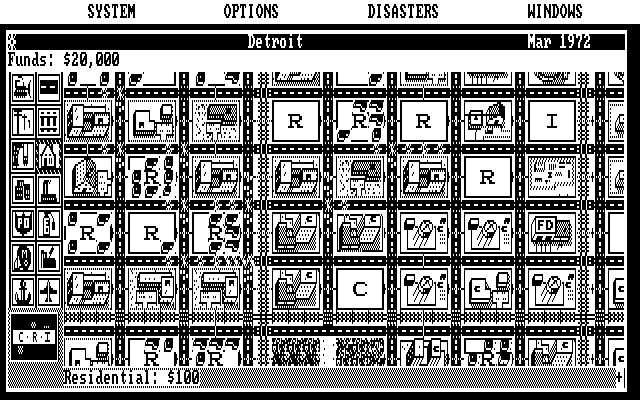
\includegraphics[width=\linewidth]{../data/figures/SimCity.png}
    \caption{SimCity in 640×200 monochrome}
    \label{fig:simcity}
  \end{subfigure}
  \caption{The IBM Colour Graphics Adapter (CGA) and its 16-colour palette.}
  \label{fig:cga-examples}
\end{figure}

% ------------------------------------------------------------------
\section{Use Cases: Early Game Graphics}
\label{sec:usecases}

Console and arcade artists faced the same constraint: a small palette and low
resolution. But are tasked with creating a visually rich experience.
The Sega Mega Drive (Genesis) offered a 9-bit palette of 512
colours, of which only a limited number could be shown at once. Artists in
games such as \emph{Sonic the Hedgehog} used checkerboard patterns of two
colours; on a CRT television connected by composite video, the signal
blurred the pattern into an apparent third colour or a semi-transparent
effect (a commonly cited example is the waterfalls of Green Hill Zone).

\todo{Verify details and cite a source.}

\begin{figure}[htbp]
  \centering
  
\includegraphics[width=0.20\textwidth]{../data/images/Sonic.png}
  \caption{Sonic the Hedgehog (1991) on the Sega Mega Drive}
  \label{fig:sonic}
\end{figure}

Dithering also served monochrome displays: Atkinson's algorithm
(Section~\ref{sec:atkinson}) was written for the original Apple Macintosh,
whose screen was strictly one bit per pixel.

\newpage

% ------------------------------------------------------------------
\section{The Primitive Approach: Nearest Colour}
\label{sec:nearest}

You might think, \textit{why do we need dithering?} 
\textit{Why can't we just quantise the image to the nearest colour in the palette?} 
Let's explore that.
The simplest strategy maps every pixel independently to the closest palette colour.
With palette $P$ and pixel $p=(r,g,b)$,
\begin{equation}
  \operatorname{map}(p) = \arg\min_{c\in P}
  \sqrt{(r-c_r)^2 + (g-c_g)^2 + (b-c_b)^2}.
\end{equation}
For two grayscale levels this reduces to thresholding at 128.
\bigskip   % \smallskip \medskip \bigskip
%\paragraph{Remark (choice of distance).}
%Euclidean distance is used rather than cosine similarity. Cosine similarity compares
%only the \emph{direction} of two colour vectors and ignores their magnitude,
%so $(255,0,0)$ and $(128,0,0)$ would be considered identical even though one is much darker.

Take a look at the example in Figure \ref{fig:apple_nearest_colour}.
The original image of an apple is quantised to different levels of quantisation, 10, 5, and 2.
You can see that as $L$ decreases, the image loses more and more information.
At level 10, the image is still recognisable, but at level 5, the image is starting to lose its details.
Notice the banding at the center of the apple as well as on the leaf,
the difference shades of green or red are lost, its more apparent where certain pixels are
mapped to the same colour and its easier to recognise the grainy texture of pixalized images. 
At level 2, its evident that the image has lost a lot of information,
its a day and night difference compared to the original image.
Because of the quantisation error, the original color of the apple is lost, its misrepresented
and is an entirely different shade of red, and the image looks flat and unnatural.

\begin{figure}[htbp]
  \centering
  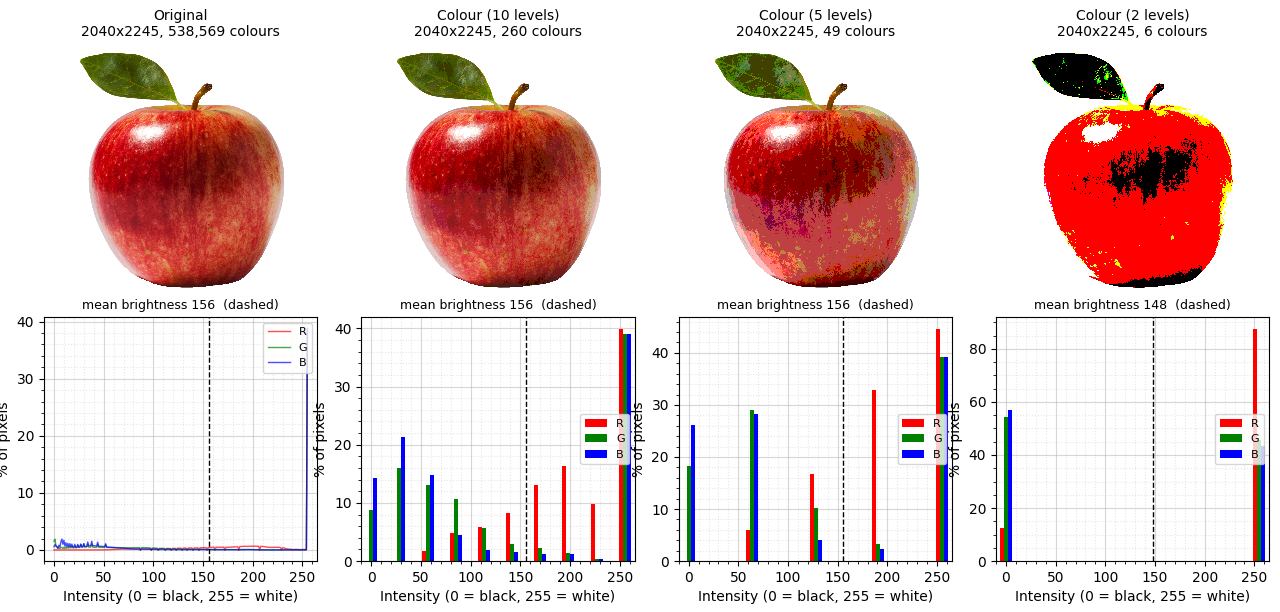
\includegraphics[width=0.95\textwidth]{../output/Section_4/Apple_1.png}
  \caption{Nearest colour mapping of an apple to different levels of quantisation}
  \label{fig:apple_nearest_colour}
\end{figure}

\begin{figure}[htbp]
  \centering
  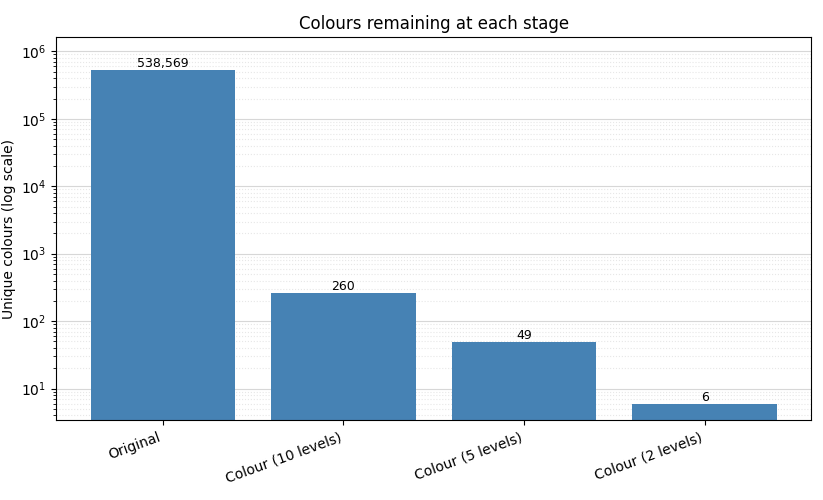
\includegraphics[width=0.55\textwidth]{../output/Section_4/Apple_2.png}
  \caption{Bar chart of the number of distinct colours in the original and the quantised images}
  \label{fig:apple_bar_chart}
\end{figure}

\newpage

The bar chart in Figure \ref{fig:apple_bar_chart} shows the number of distinct colours
in the quantised images drops logarithmically as $L$ decreases.
It terms of numbers, the original image has 538,569 distinct colours,
while the all quantised images have less literally than 0.048\% of the original number of distinct colours.
Although its apparent for levels 5 and 2, the color information is significantly reduced,
its actually not as apparent in level 10, the number of distinct colours is still reduced by 99.95\%,
but the image still looks recognisable and retains a lot of its original information.
This ultimately is an optical illusion and has to do with how the human eye perceives colour and light,
the image looks recognisable but we know the color information is significantly reduced,
what we perceive as a single shade of colour is actually a combination of different distinct colours.

\medskip   % \smallskip \medskip \bigskip

Here's another example of nearest colour mapping in Figure \ref{fig:rock}.
The original image of a rock is mostly grey, with some brown and blue tones.
When mapped to a 8-colour palette, the image loses a lot of its original information;
grey areas are mapped to either black or white,
and those small specks of brown and blue tones are now very apparent. 

\begin{figure}[htbp]
  \centering
  \begin{subfigure}[t]{0.40\textwidth}
    \raisebox{-\height}{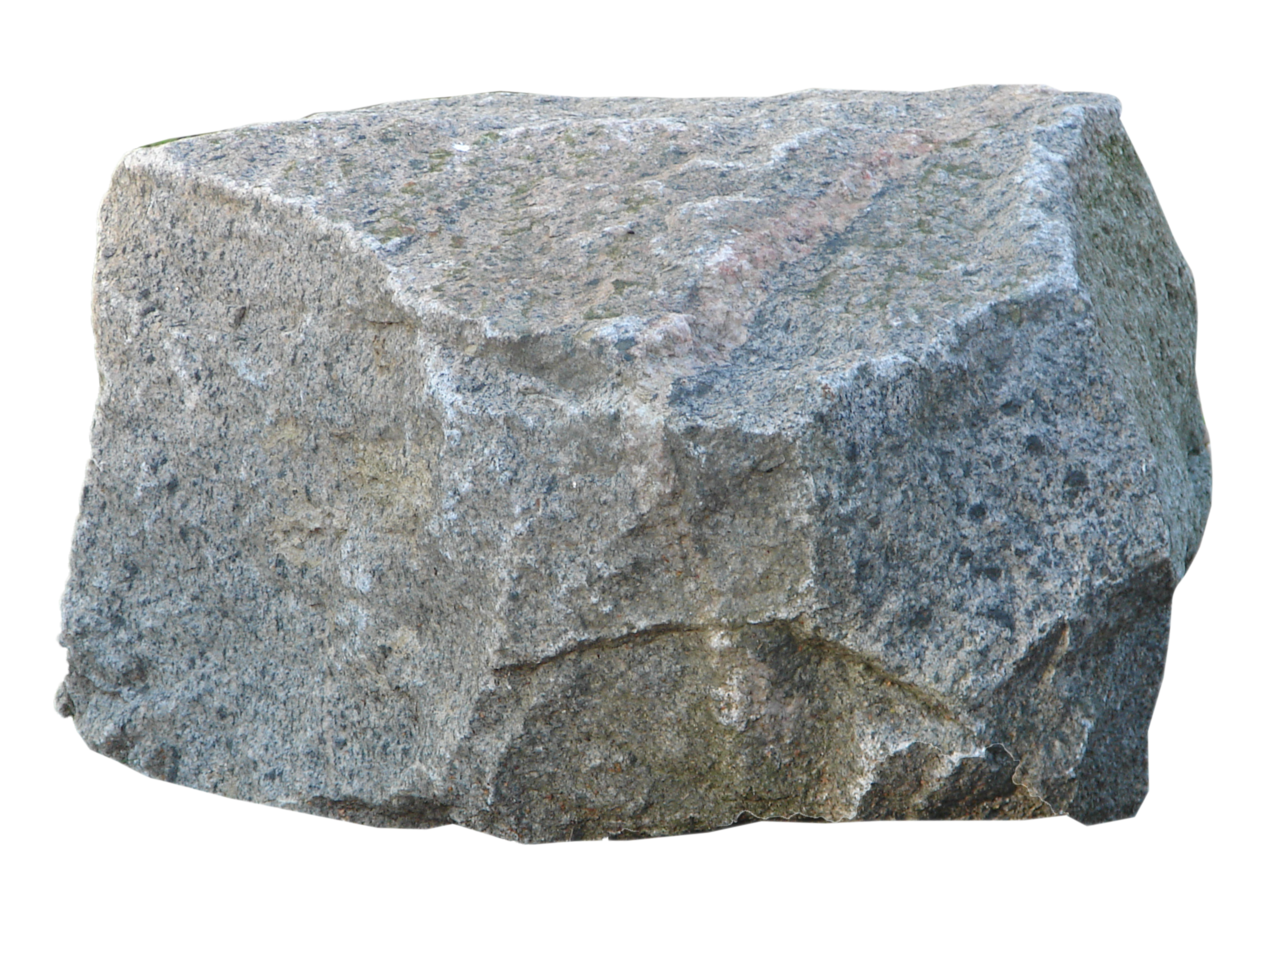
\includegraphics[width=\linewidth]{../data/images/Rock.png}}
    \caption{Original image of a rock}
    \label{fig:rock_original}
  \end{subfigure}
  \begin{subfigure}[t]{0.40\textwidth}
    \raisebox{-\height}{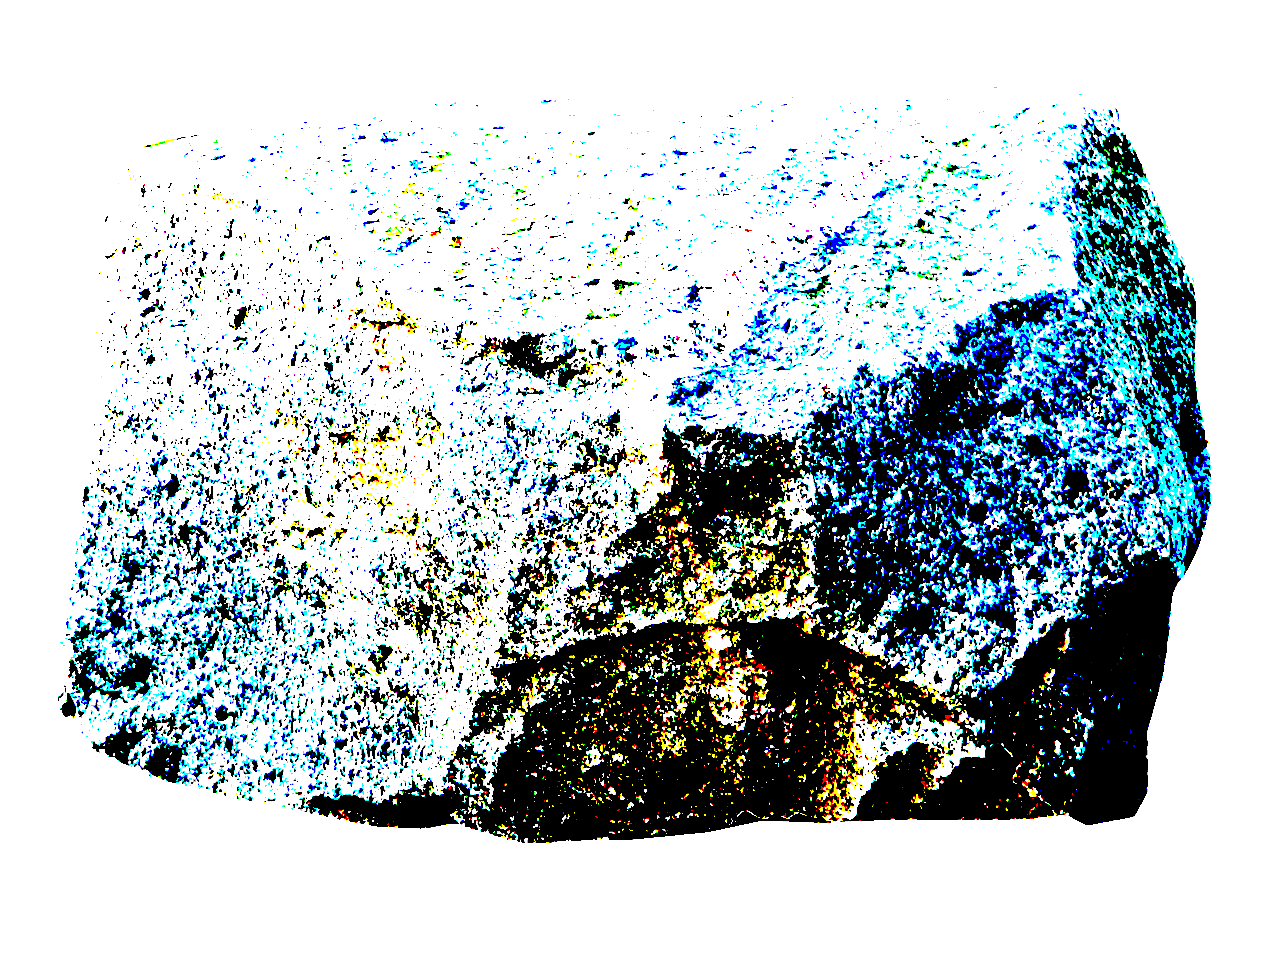
\includegraphics[width=\linewidth]{../output/Section_4/Rock_1.png}}
    \caption{Mapped to a 8-colour palette}
    \label{fig:rock1}
  \end{subfigure}
  \caption{Nearest colour mapping of a rock}
  \label{fig:rock}
\end{figure}

Nearest-colour mapping discards the error entirely.
Smooth gradients collapse into flat regions with hard edges (\emph{banding} or \emph{contouring}),
and large areas of similar tone become a single solid colour.
The algorithms in Section~\ref{sec:algorithms} fix this by \emph{remembering} the error.
\todo{Insert a threshold-versus-dithered comparison figure.}

\newpage

% ------------------------------------------------------------------
\section{Dithering Algorithms}
\label{sec:algorithms}
In layman's terms, dithering is a technique used to create the illusion of more colors
in an image by mixing pixels of different colors together.
There are many ways to dither an image, but they all share the same basic idea:
\begin{enumerate}
  \item Quantise the current pixel to the nearest palette colour.
  \item Compute the quantisation error.
  \item Distribute the error to neighbouring pixels that have not yet been processed.
  \item Repeat until all pixels have been processed.
\end{enumerate}
Dithering algorithms can be broadly classified into two categories:
point processing and error diffusion.

\subsection{Point processing}
Point processing algorithms operate on each pixel independently,
without considering the neighbouring pixels.
The advantage of point processing is that it is fast and simple to implement.
The disadvantage is that it can produce a grainy texture
and does not preserve the mean brightness of the image.

\subsubsection{Random dithering}
The simplest method is to add random noise to each pixel before quantisation,
which breaks up the banding but produces a grainy texture.
We add a random value $r\in[-\Delta/2, \Delta/2]$ to each pixel before quantisation:
\begin{equation}
  \text{new} = q(\text{old} + r), \qquad r \sim \mathcal{U}\!\left[-\frac{\Delta}{2}, \frac{\Delta}{2}\right].
\end{equation}
The reason why this works is that the quantisation error is uniformly distributed
in $[-\Delta/2, \Delta/2]$, so adding a random value from the same range will cancel out
the error on average.
\todo{Add a gradient figure}
\todo{Compare threshold and random dithering}
Let's say we have an image of a gradient from black to white,
and we want to quantise it to 2 levels (black and white).
If we use nearest colour mapping, the gradient will be quantised to either black or white,
which produces a banding effect where we have a clear threshold.
However, if we add random noise to each pixel before quantisation,
the gradient will be quantised to a mix of black and white pixels,
which creates that illusion of a smooth gradient.

\todo{Add intensity histogram of the original and dithered images}

\newpage

Take a look at Figure \ref{fig:tennis-balls}, we'll random dither a greyscale image of tennis balls
$L={2,3,9}$. 

\begin{figure}[htbp]
  \centering
  \begin{subfigure}[t]{0.45\textwidth}
    {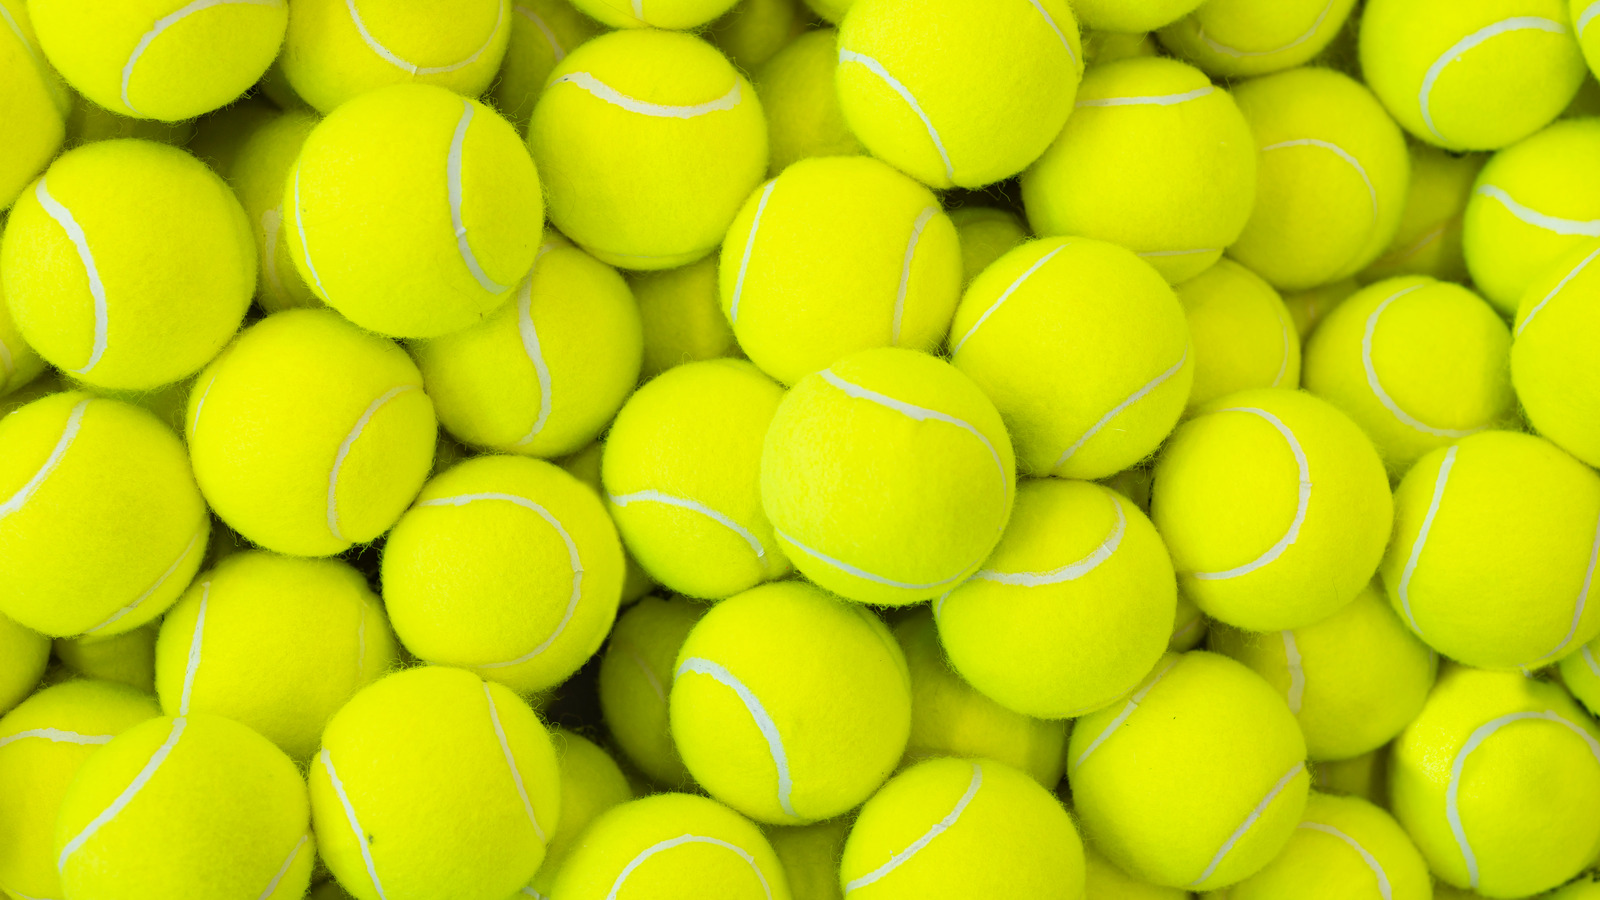
\includegraphics[width=\linewidth]{../data/images/Tennis-Balls.jpg}}
    \caption{Original}
    \label{fig:tennis-balls-original}
  \end{subfigure}
  \hspace{0.04\textwidth}%
  \begin{subfigure}[t]{0.45\textwidth}
    {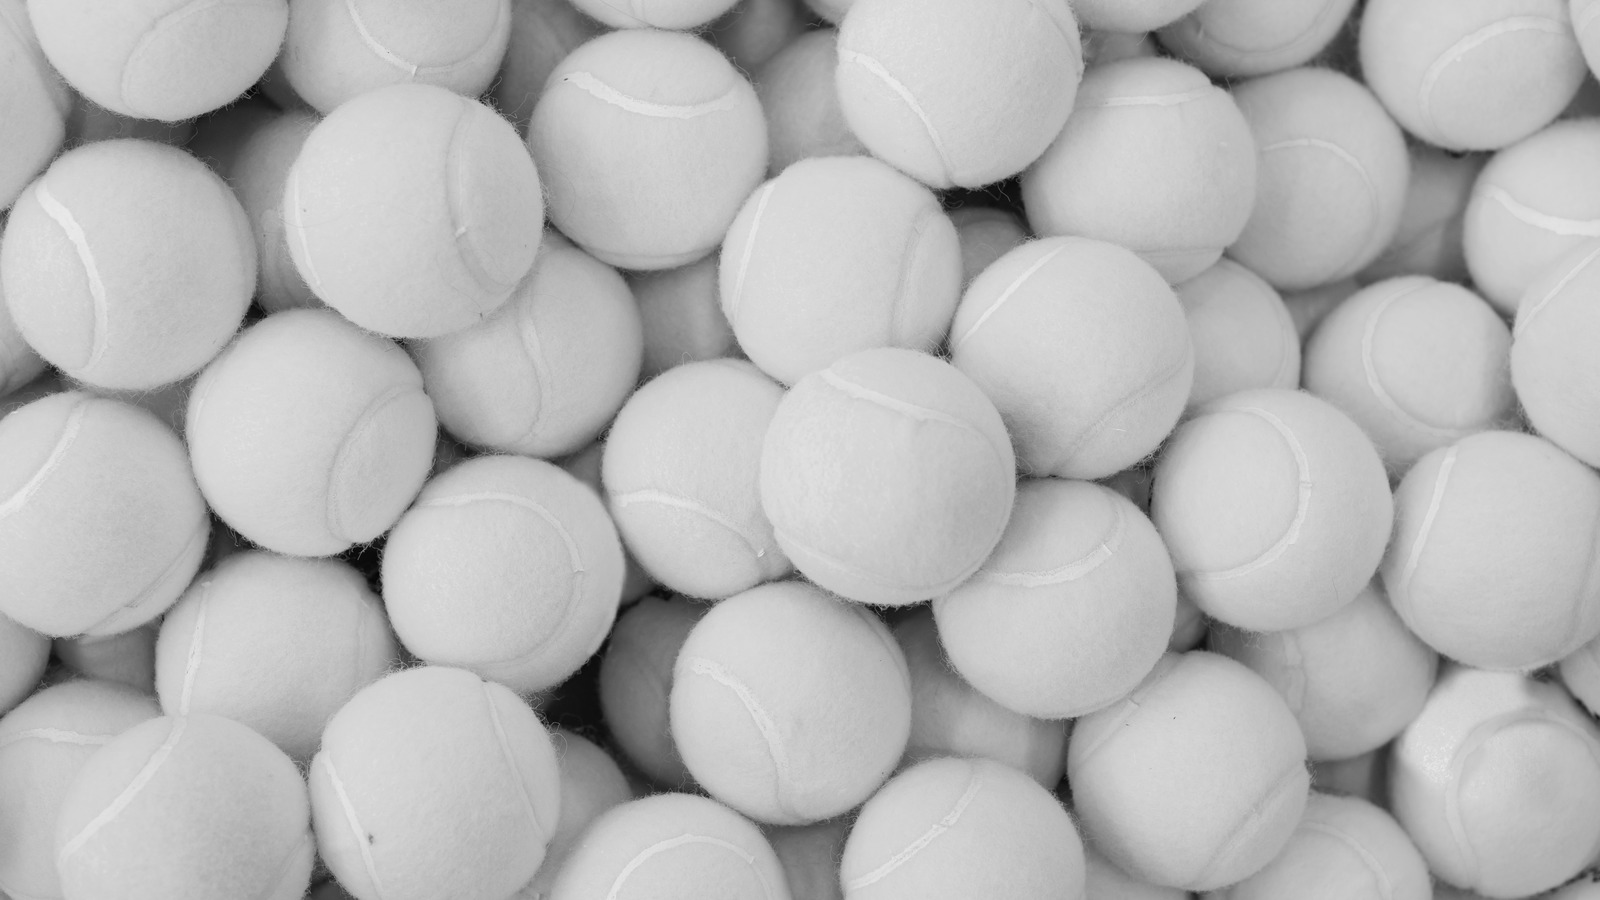
\includegraphics[width=\linewidth]{../output/Section_5_1/Tennis-Balls_greyscaled.png}}
    \caption{Greyscale}
    \label{fig:tennis-balls-grayscale}
  \end{subfigure}

  \begin{subfigure}[t]{0.31\textwidth}
    {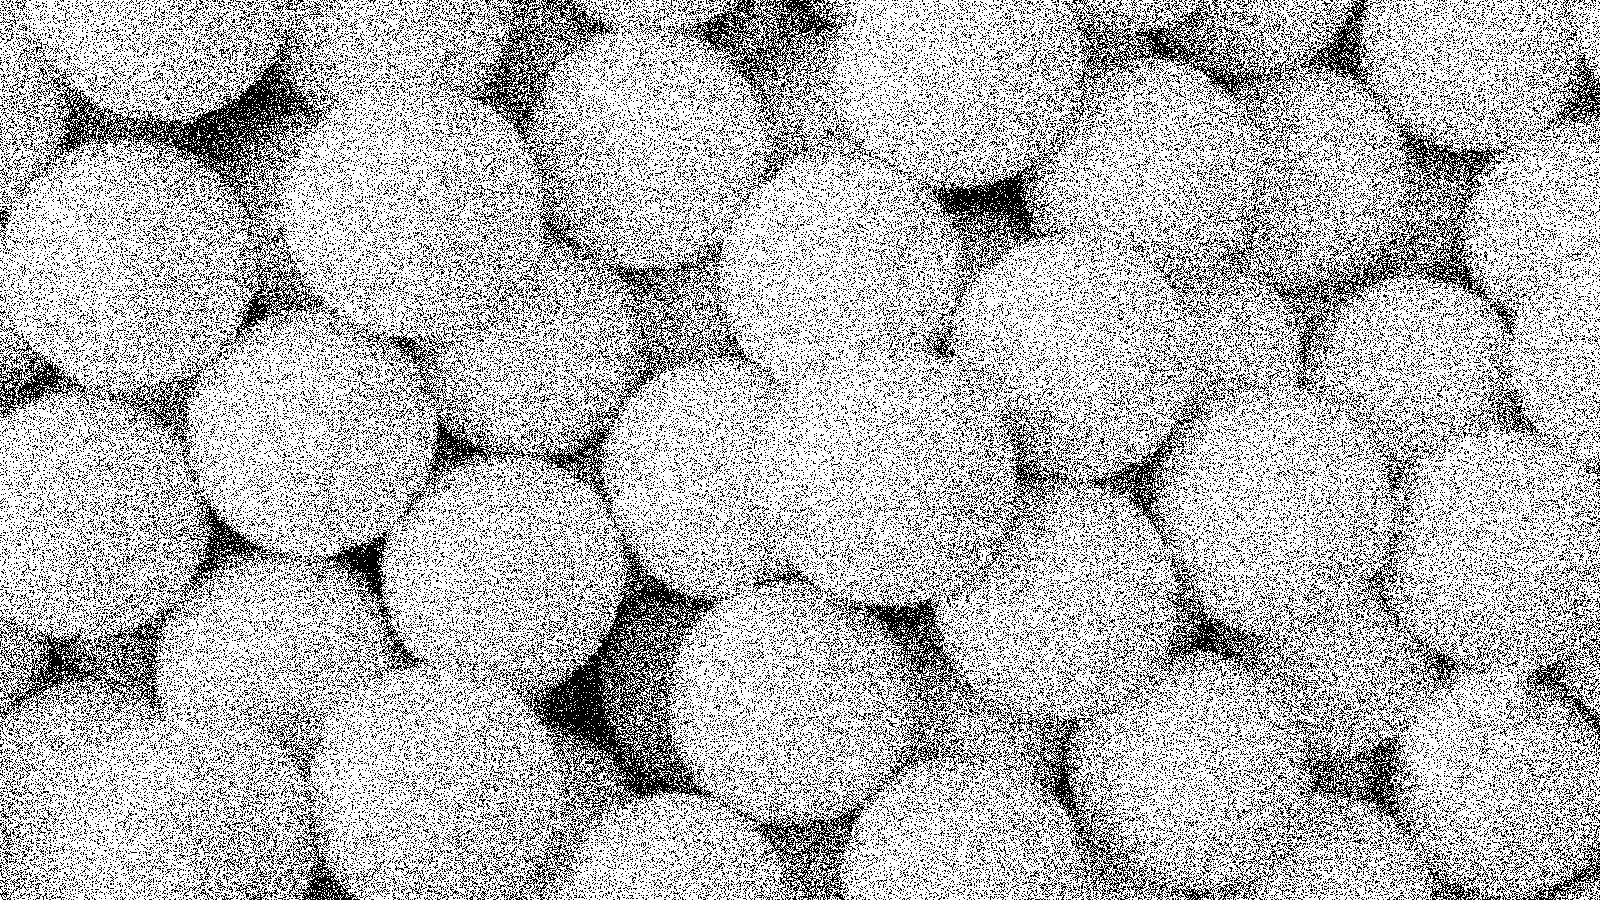
\includegraphics[width=\linewidth]{../output/Section_5_1/Tennis-Balls_random2.png}}
    \caption{Random Dithering (Levels=2)}
    \label{fig:tennis-balls-random2}
  \end{subfigure}
  \begin{subfigure}[t]{0.31\textwidth}
    {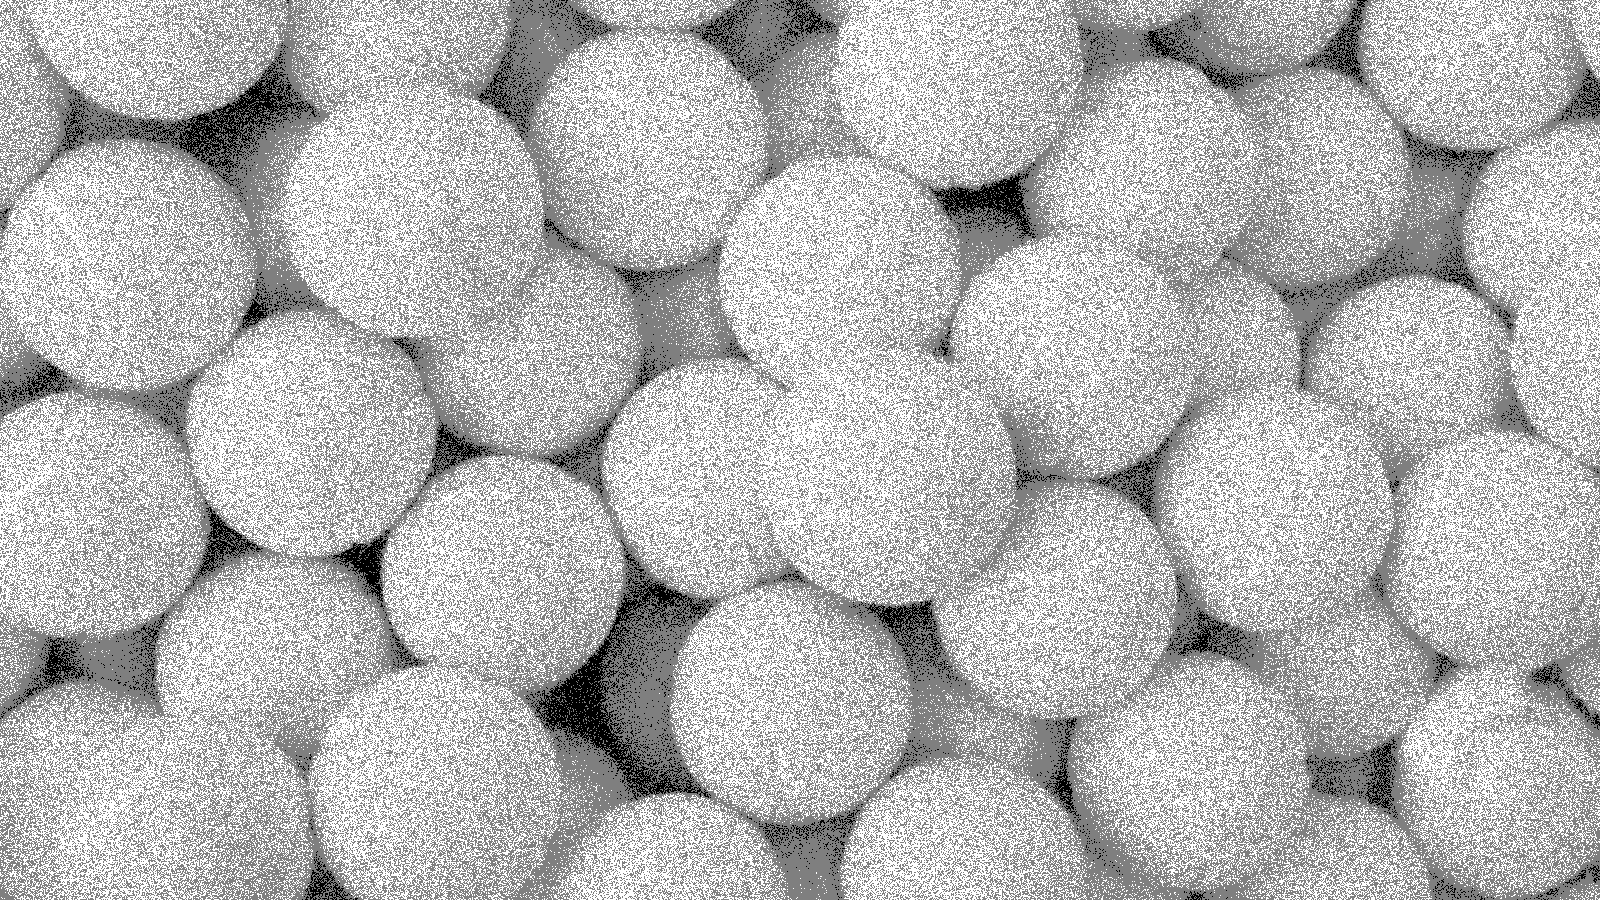
\includegraphics[width=\linewidth]{../output/Section_5_1/Tennis-Balls_random3.png}}
    \caption{Random Dithering (Levels=3)  }
    \label{fig:tennis-balls-random3}
  \end{subfigure}
  \begin{subfigure}[t]{0.31\textwidth}
    {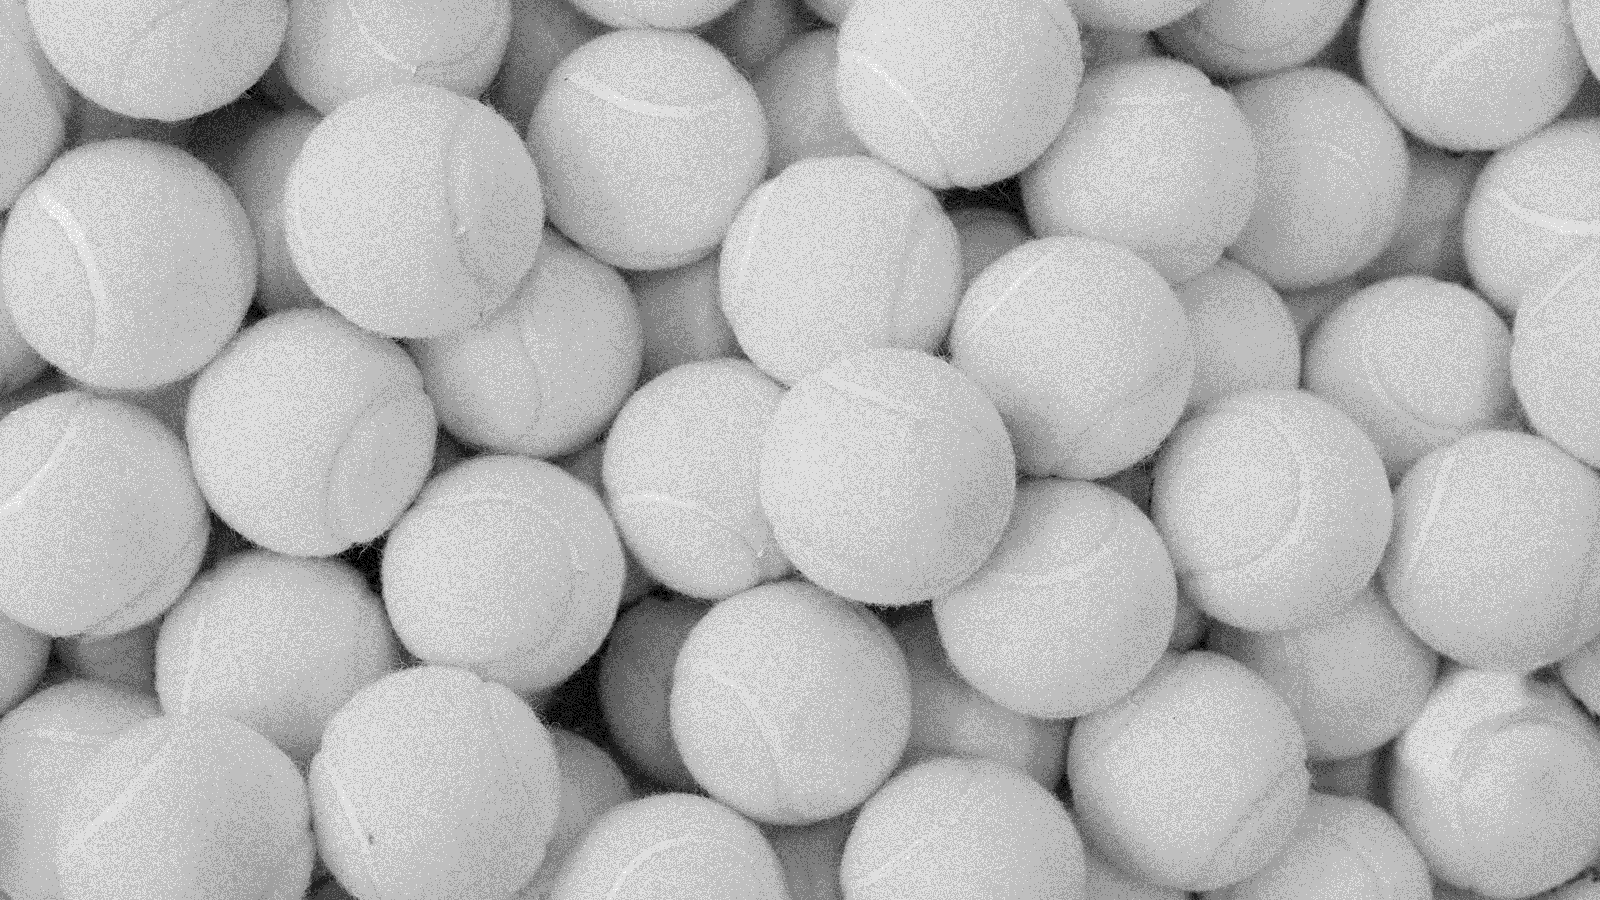
\includegraphics[width=\linewidth]{../output/Section_5_1/Tennis-Balls_random9.png}}
    \caption{Random Dithering (Levels=9)}
    \label{fig:tennis-balls-random9}
  \end{subfigure}
  \caption{Random dithering applied to greyscale image of tennis balls}
  \label{fig:tennis-balls}
\end{figure}

The reason why we use a greyscale image is that it allows us to focus on
the dithering effect without the distraction of colour.
If you're curious to see how random dithering works on a coloured image,
take a look at Figure \ref{fig:yahoo} below.

\begin{figure}[htbp]
  \centering
   \begin{subfigure}[t]{0.30\textwidth}
    {
\includegraphics[width=\linewidth]{../data/images/Yahoo.png}}
    \caption{Original}
    \label{fig:yahoo-original}
  \end{subfigure}
  \hfill
  \begin{subfigure}[t]{0.30\textwidth}
    {
\includegraphics[width=\linewidth]{../output/Section_5_1/Yahoo_random2.png}}
    \caption{Random Dithering (Levels=2)}
    \label{fig:yahoo-random2}
  \end{subfigure}
  \hfill
  \begin{subfigure}[t]{0.30\textwidth}
    {
\includegraphics[width=\linewidth]{../output/Section_5_1/Yahoo_random5.png}}
    \caption{Random Dithering (Levels=5)}
    \label{fig:yahoo-random5}
  \end{subfigure}
  \caption{Random dithering applied to coloured image of Yahoo logo}
  \label{fig:yahoo}
\end{figure}

Random dithering is all about generating white-noise, and its apparent.
If you inspect Figure \ref{fig:tennis-balls-random2} the tennis ball are generally quite visible,
but the finer details are lost and are essentially replaced with the generated noise.
As we increase $L$ we find that the grain is less aparent and the original information is better retained.
The amount of noise we generate also matters.
Take a look at Figure \ref{fig:lanterns} on the next page.
As we introduce a more noise, uniform shades tend to show more noise and we get that grainy texture
instead of the smooth shade of the original image.

\begin{figure}[htbp]
  \centering
  \begin{subfigure}[t]{0.45\textwidth}
    {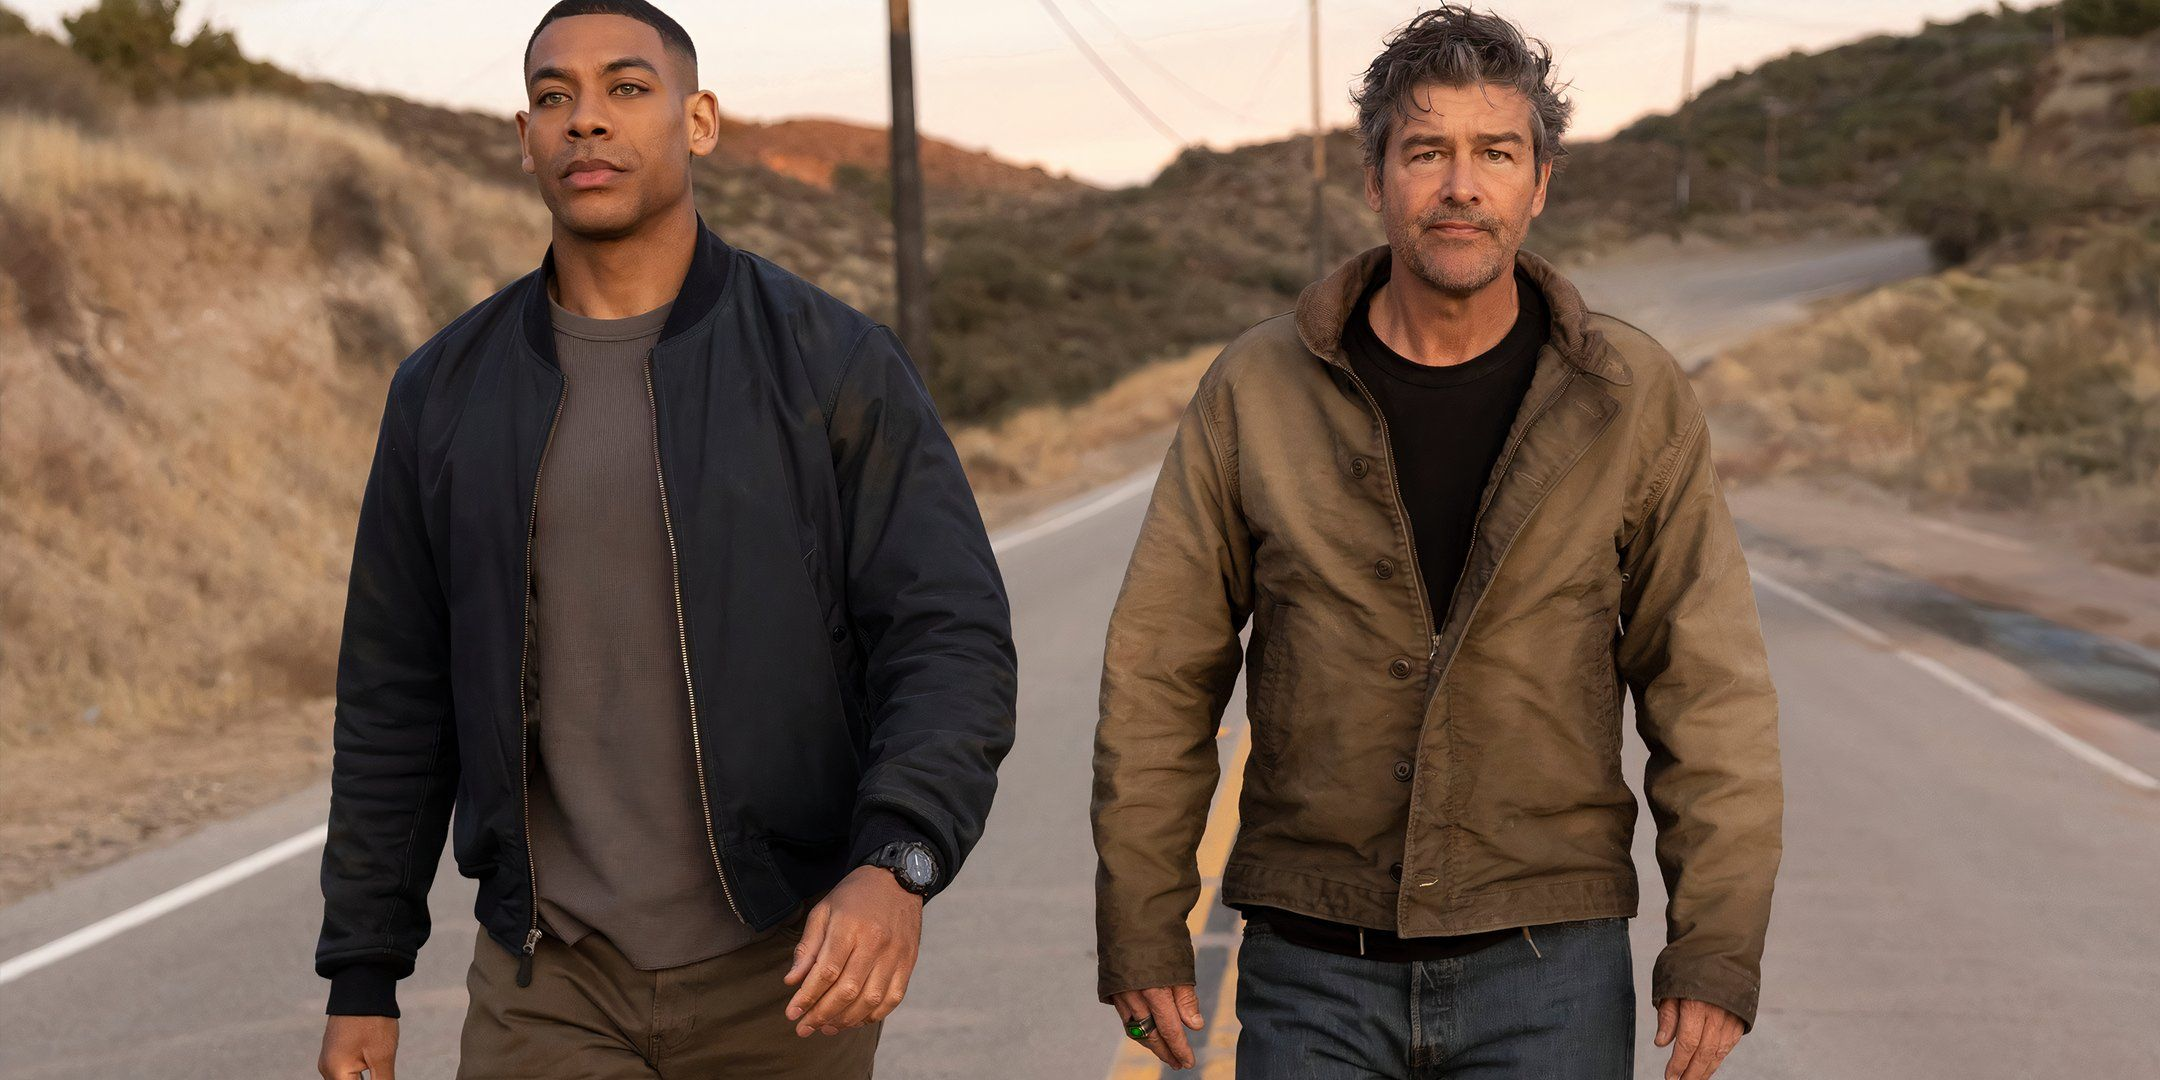
\includegraphics[width=\linewidth]{../data/images/Lanterns.jpg}}
    \caption{Original}
    \label{fig:lanterns-original}
  \end{subfigure}
  \begin{subfigure}[t]{0.45\textwidth}
    {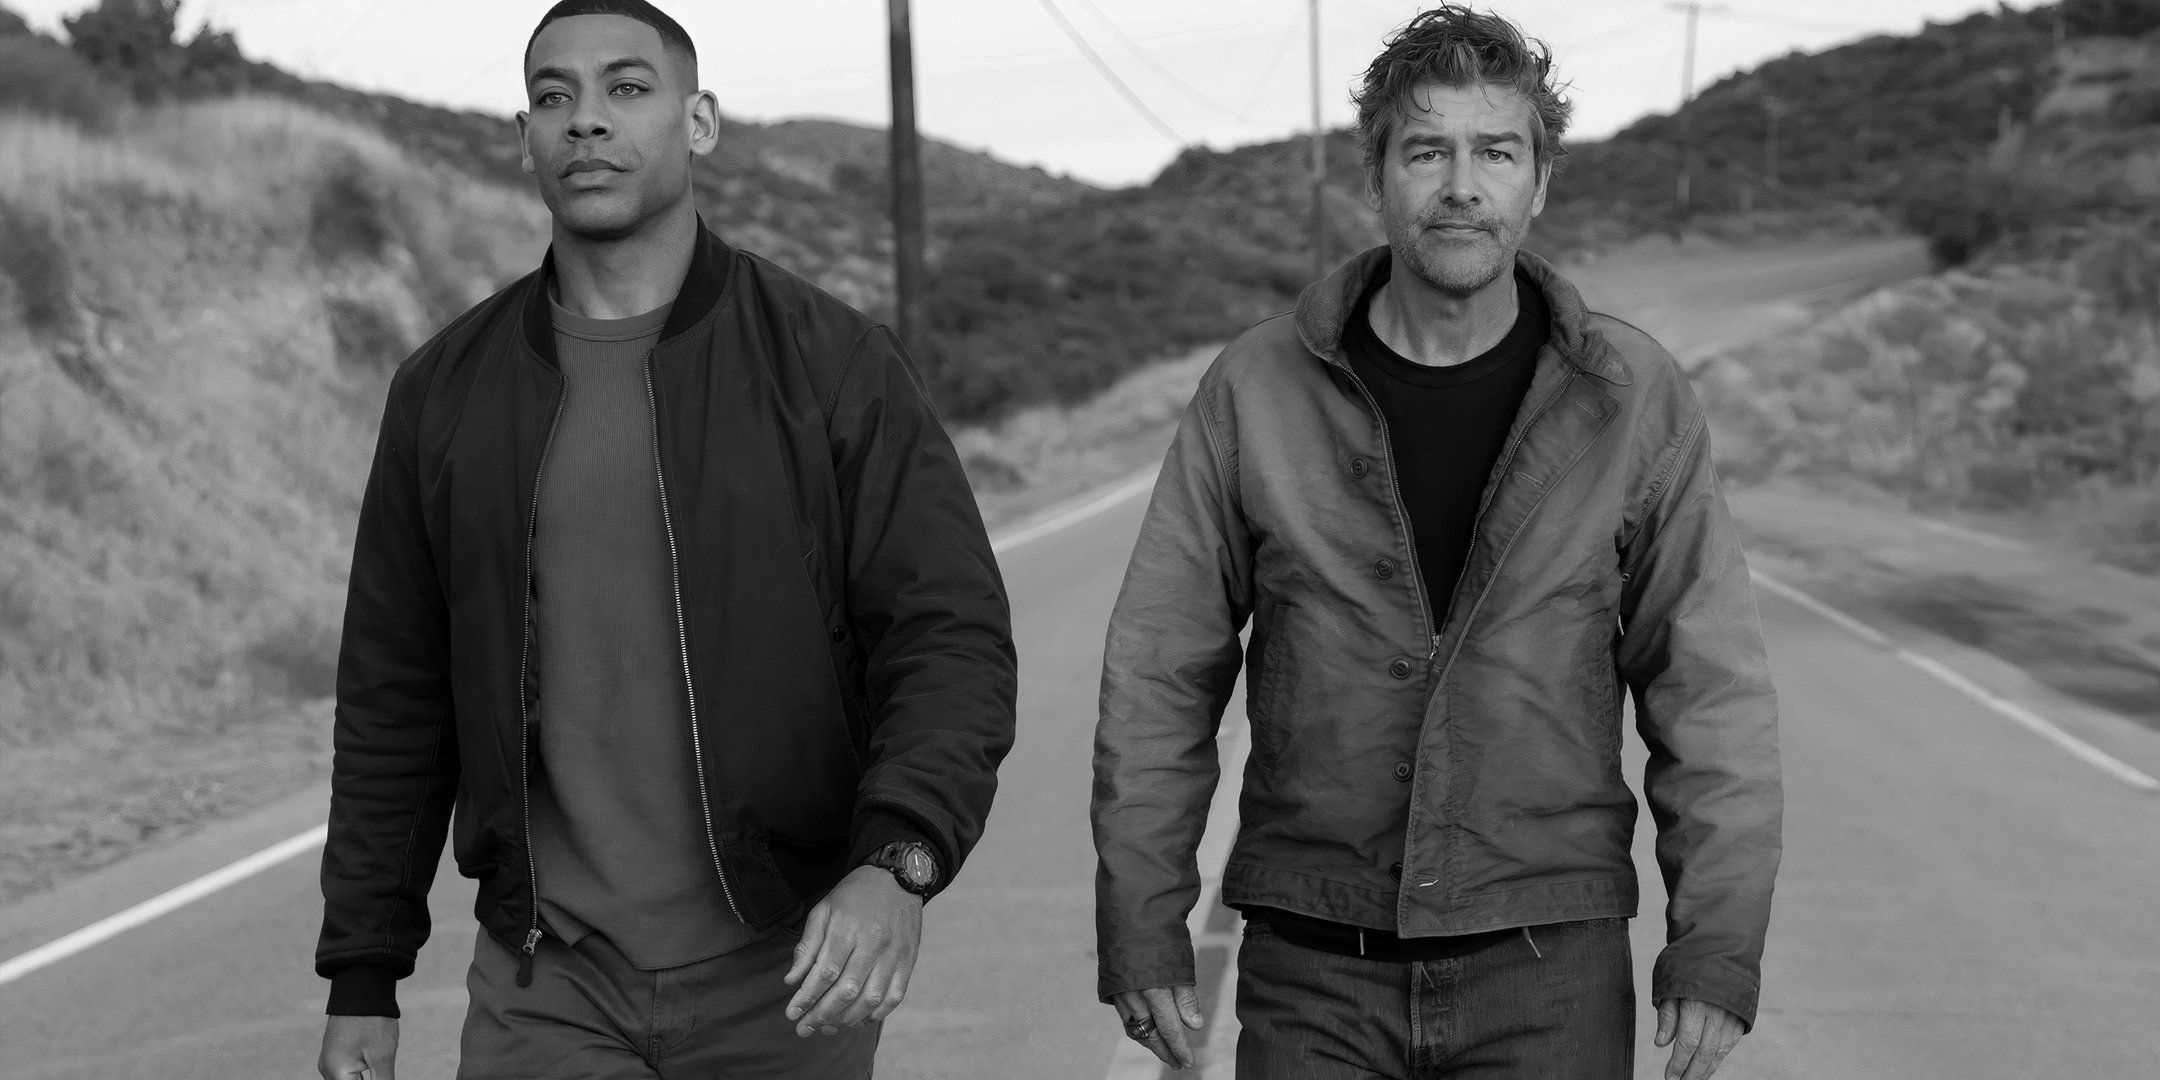
\includegraphics[width=\linewidth]{../output/Section_5_1/Lanterns_greyscaled.png}}
    \caption{Greyscale}
    \label{fig:lanterns-grayscale}
  \end{subfigure}

  \begin{subfigure}[t]{0.70\textwidth}
    {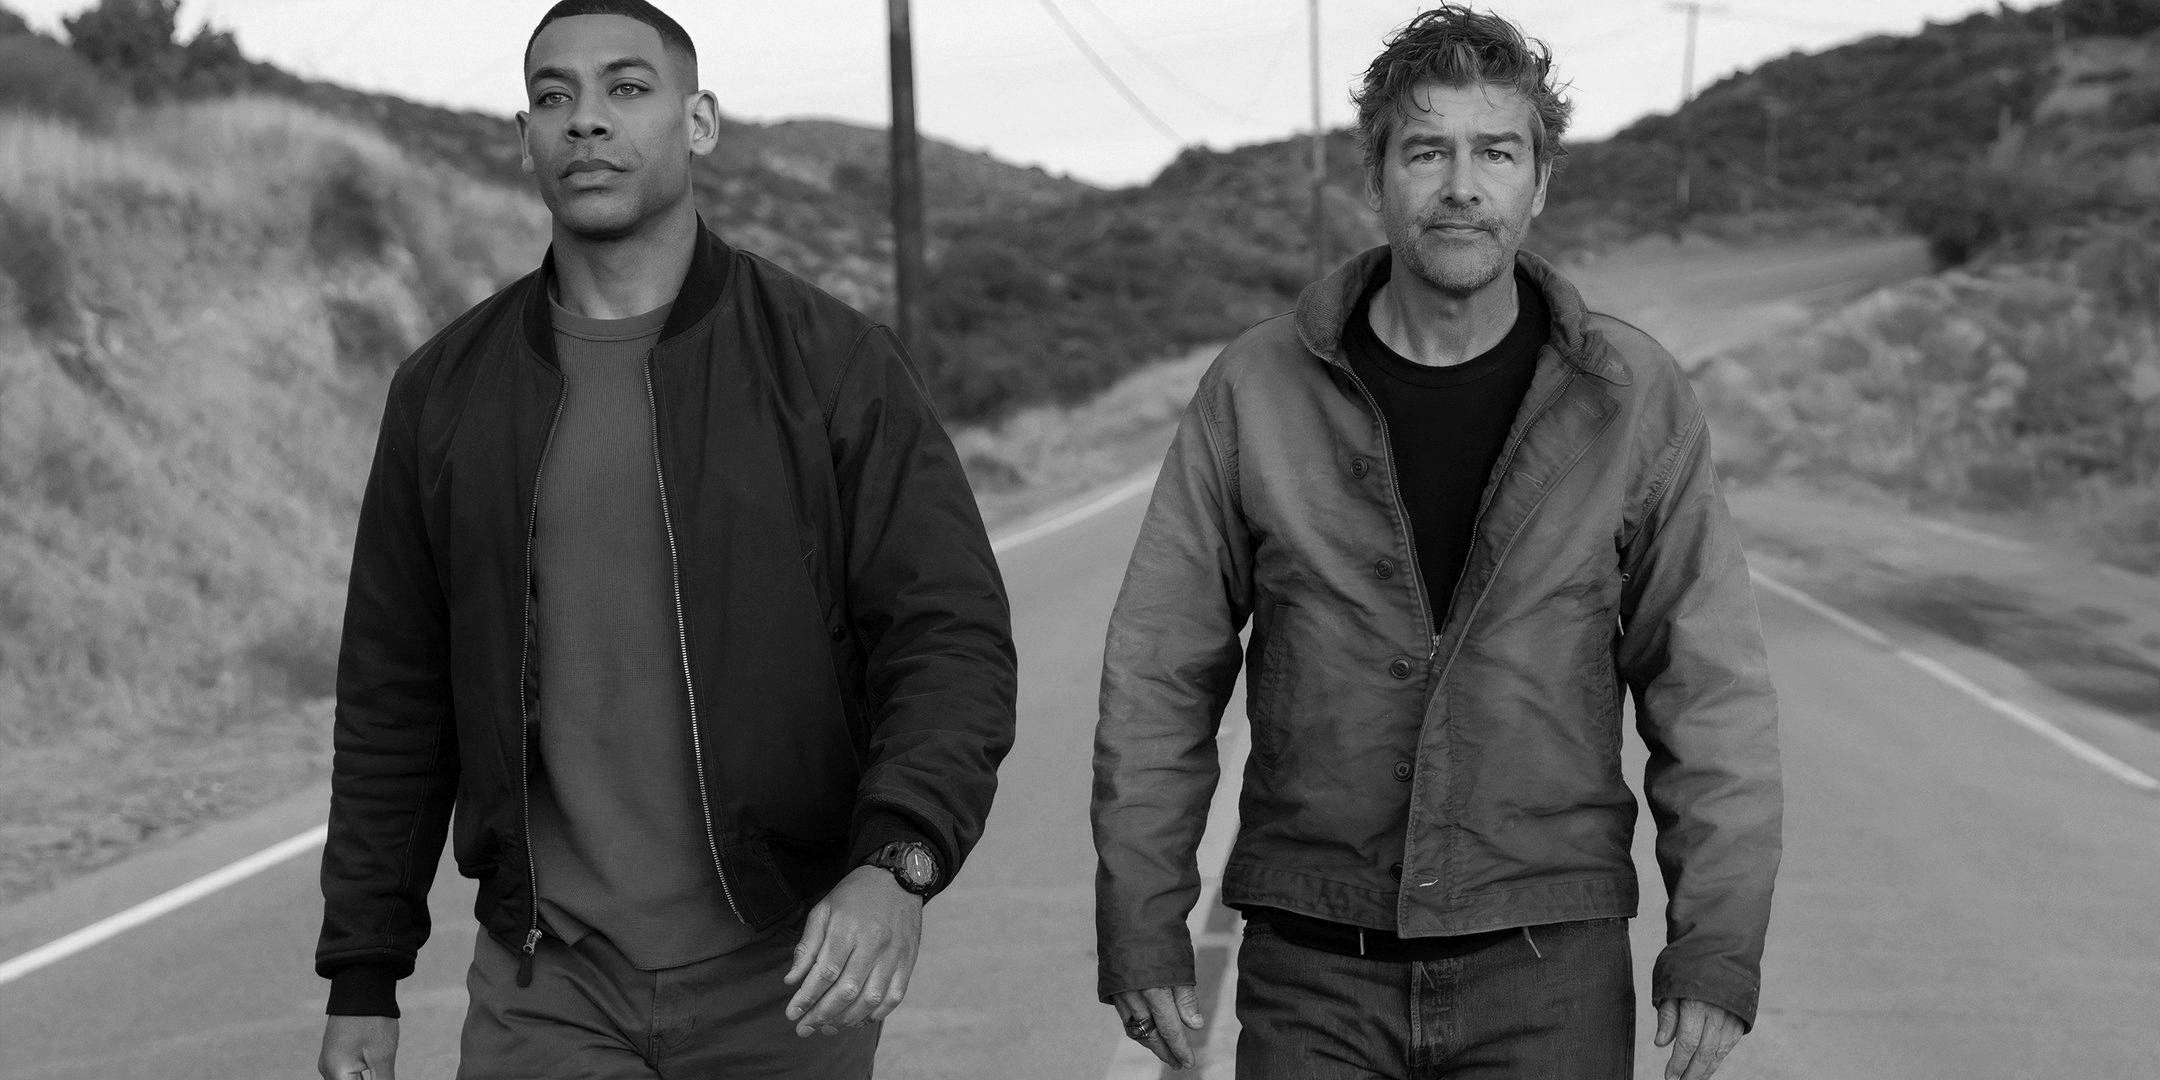
\includegraphics[width=\linewidth]{../output/Section_5_1/Lanterns_random_1.0.png}}
    \caption{Small noise}
    \label{fig:lanterns-noise-1}
  \end{subfigure}
  \begin{subfigure}[t]{0.70\textwidth}
    {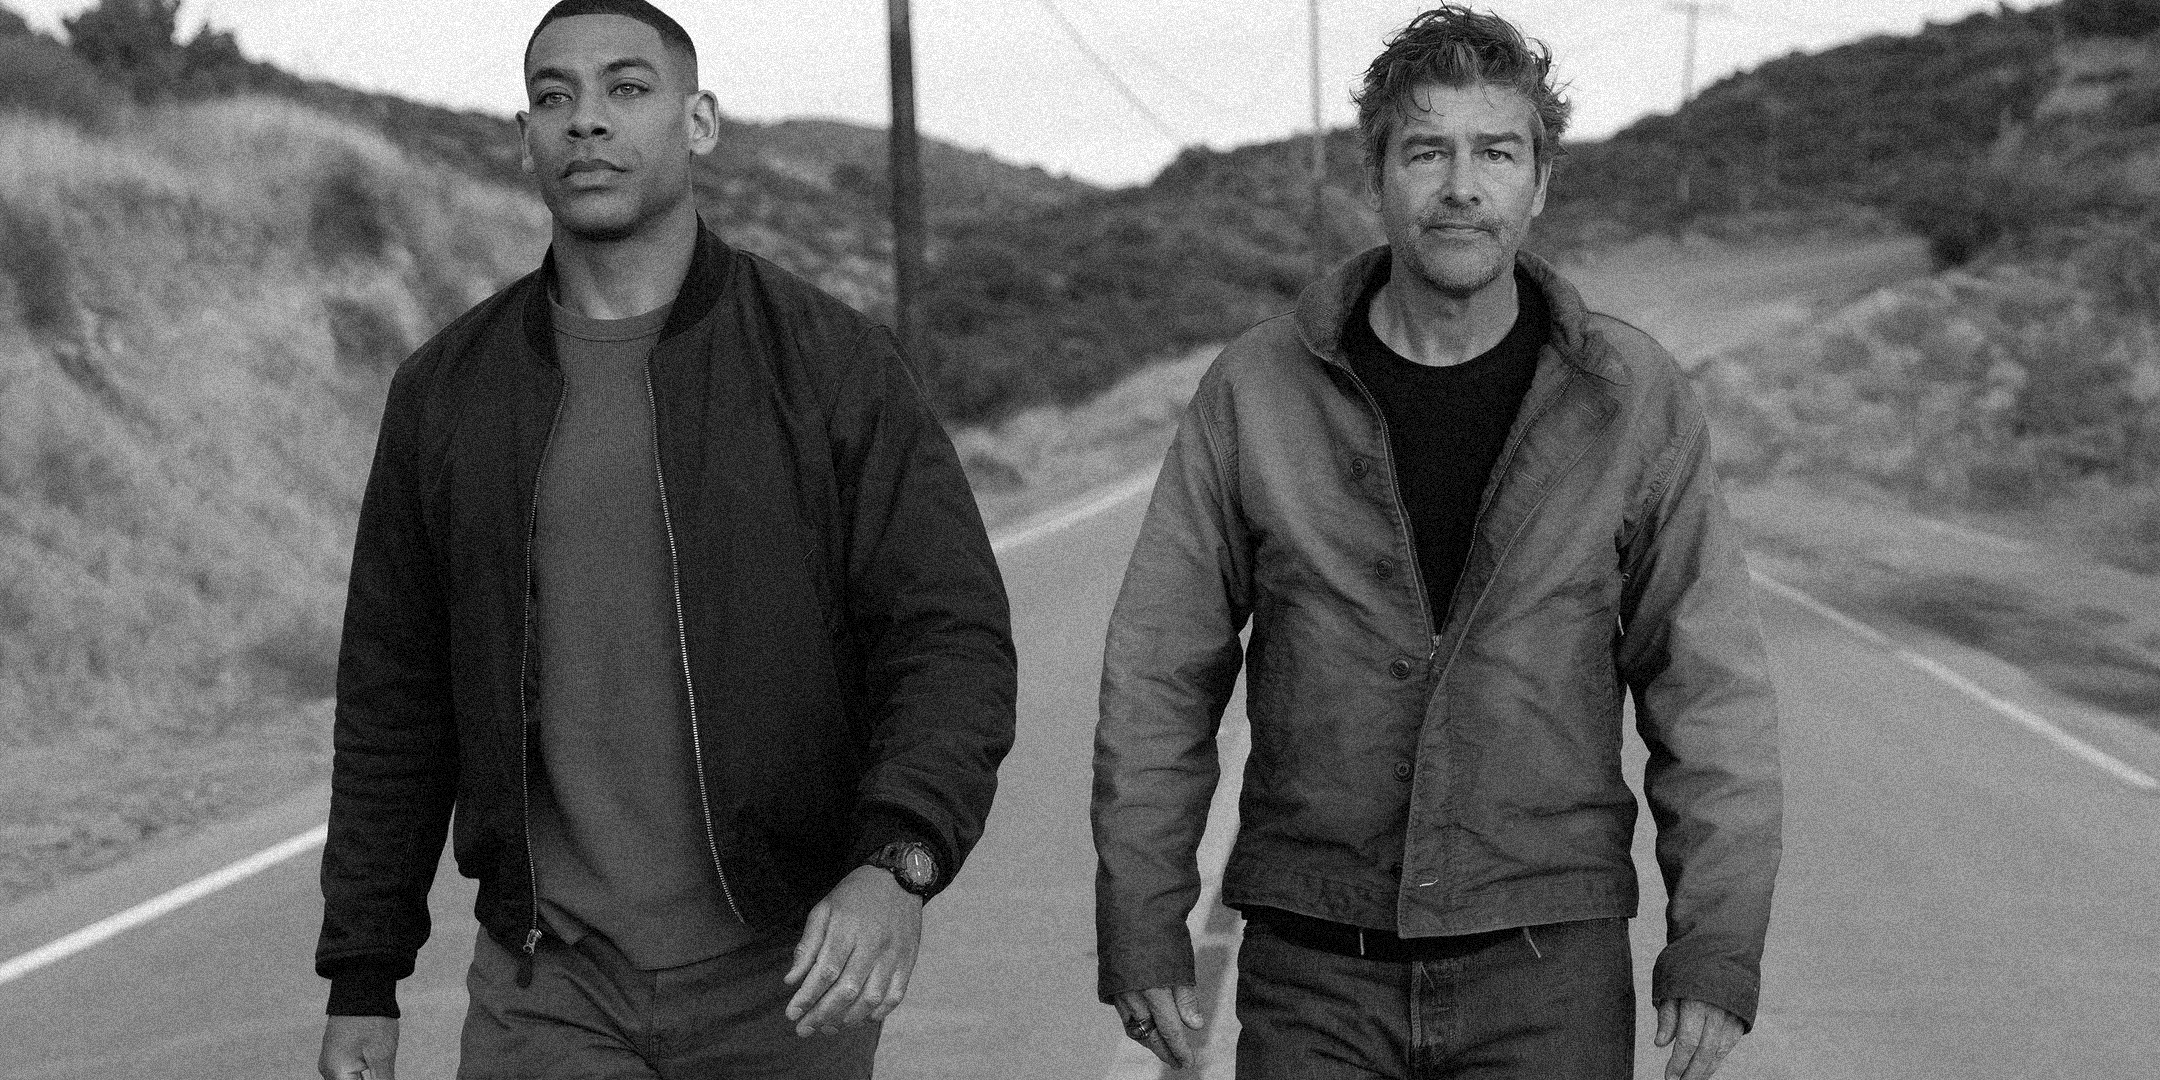
\includegraphics[width=\linewidth]{../output/Section_5_1/Lanterns_random_5.0.png}}
    \caption{Moderate noise}
    \label{fig:lanterns-noise-5}
  \end{subfigure}
  \begin{subfigure}[t]{0.70\textwidth}
    {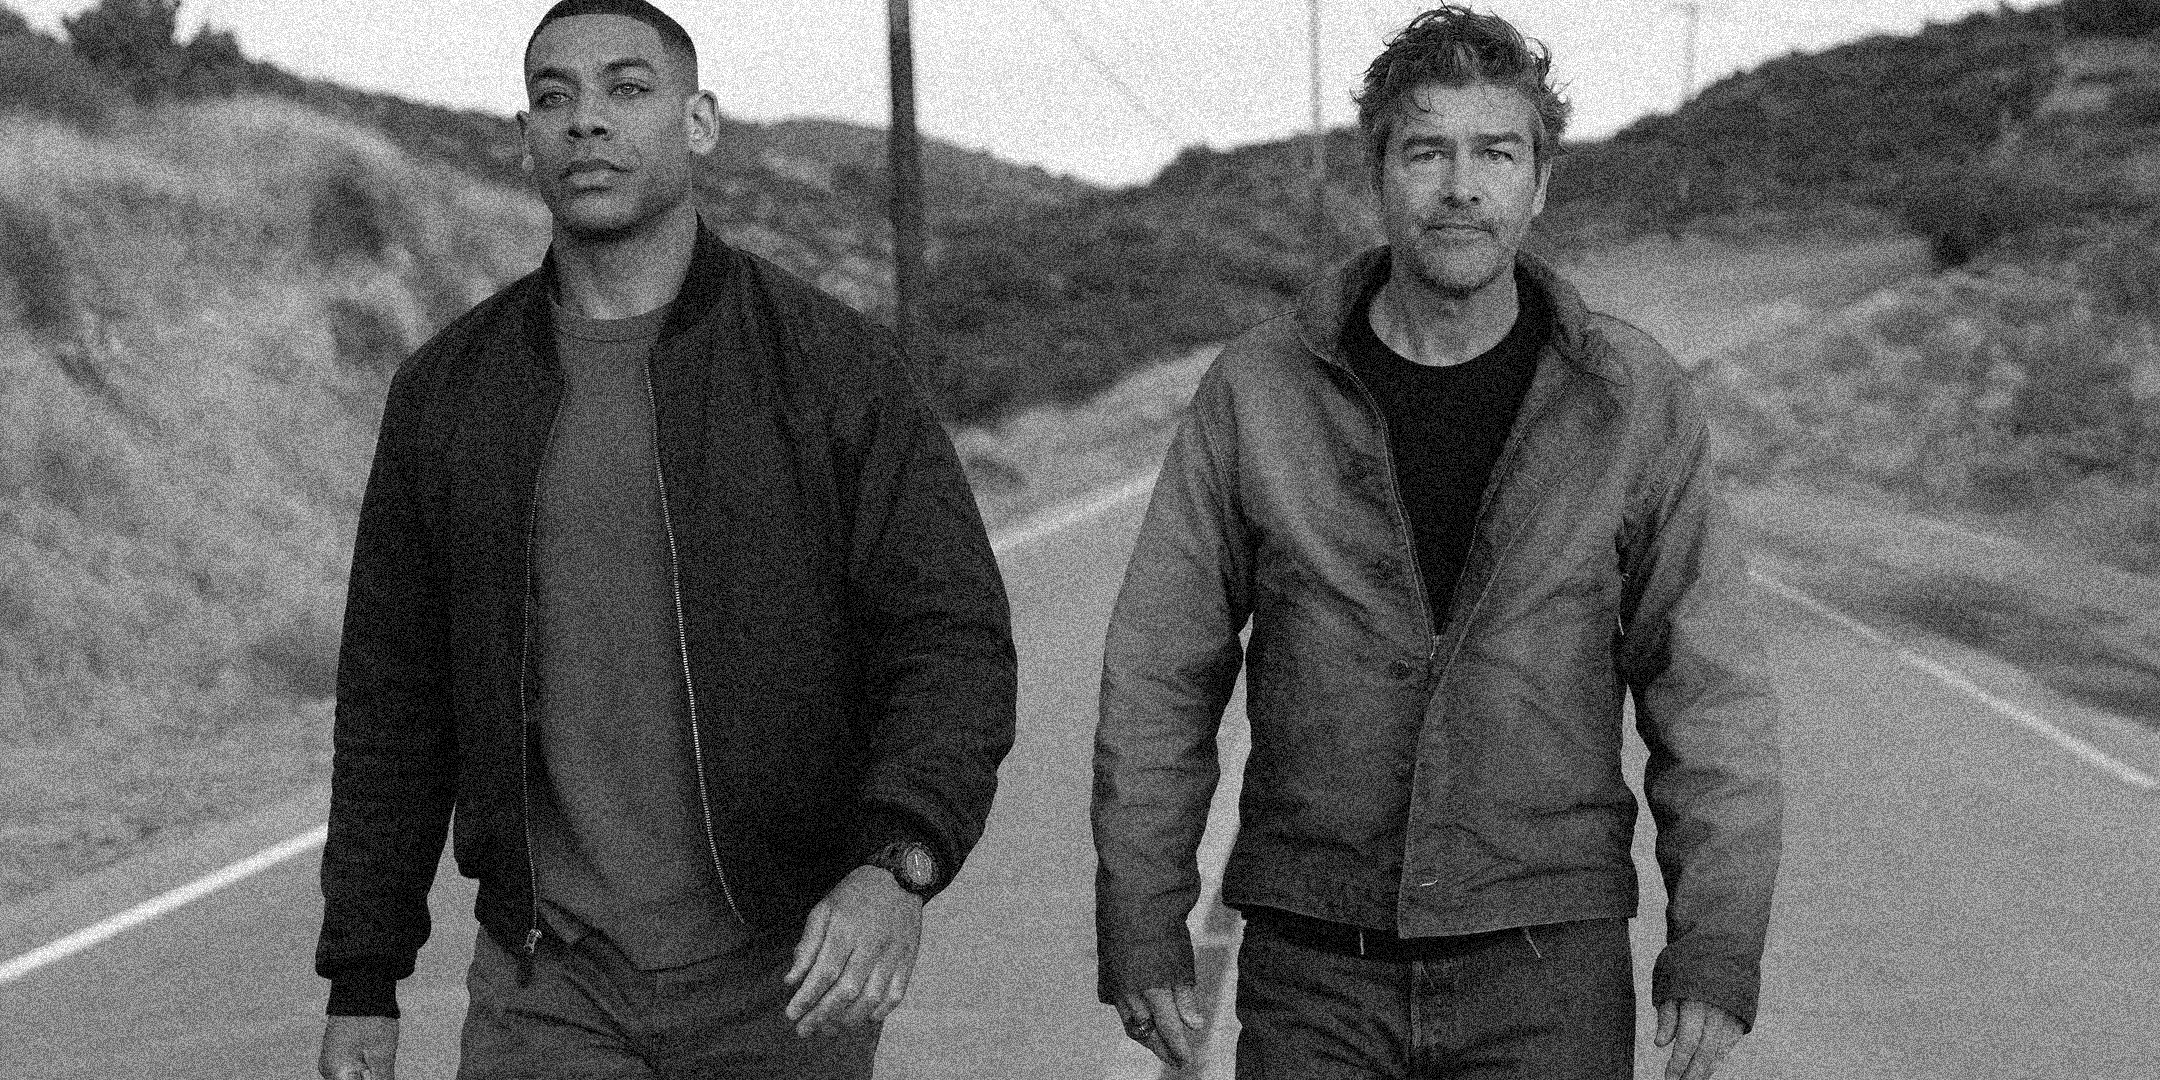
\includegraphics[width=\linewidth]{../output/Section_5_1/Lanterns_random_10.0.png}}
    \caption{Large noise}
    \label{fig:lanterns-noise-10}
  \end{subfigure}
  \caption{Random dithering applied to greyscale image of lanterns with different levels of noise}
  \label{fig:lanterns}
\end{figure}

\newpage

\subsubsection{Bayer dithering}
Bayer dithering is a more structured approach. It uses something called a 
\emph{dither matrix}to add a fixed pattern of noise to the image.
We apply a convolution of the matrix across the image to get our dithered image.
It is a type of ordered dithering that uses a threshold map to
determine which pixels to quantise to which colour.

A bayer matrix 

\newpage

\subsection{Error diffusion}
A more sophisticated approach is to use a \emph{dither matrix} to distribute the 
quantisation error in a regular pattern.
The most common method is \emph{error diffusion},
which spreads the error to neighbouring pixels that have not yet been processed.

\begin{figure}[htbp]
  \centering
  \begin{subfigure}{0.32\textwidth}
    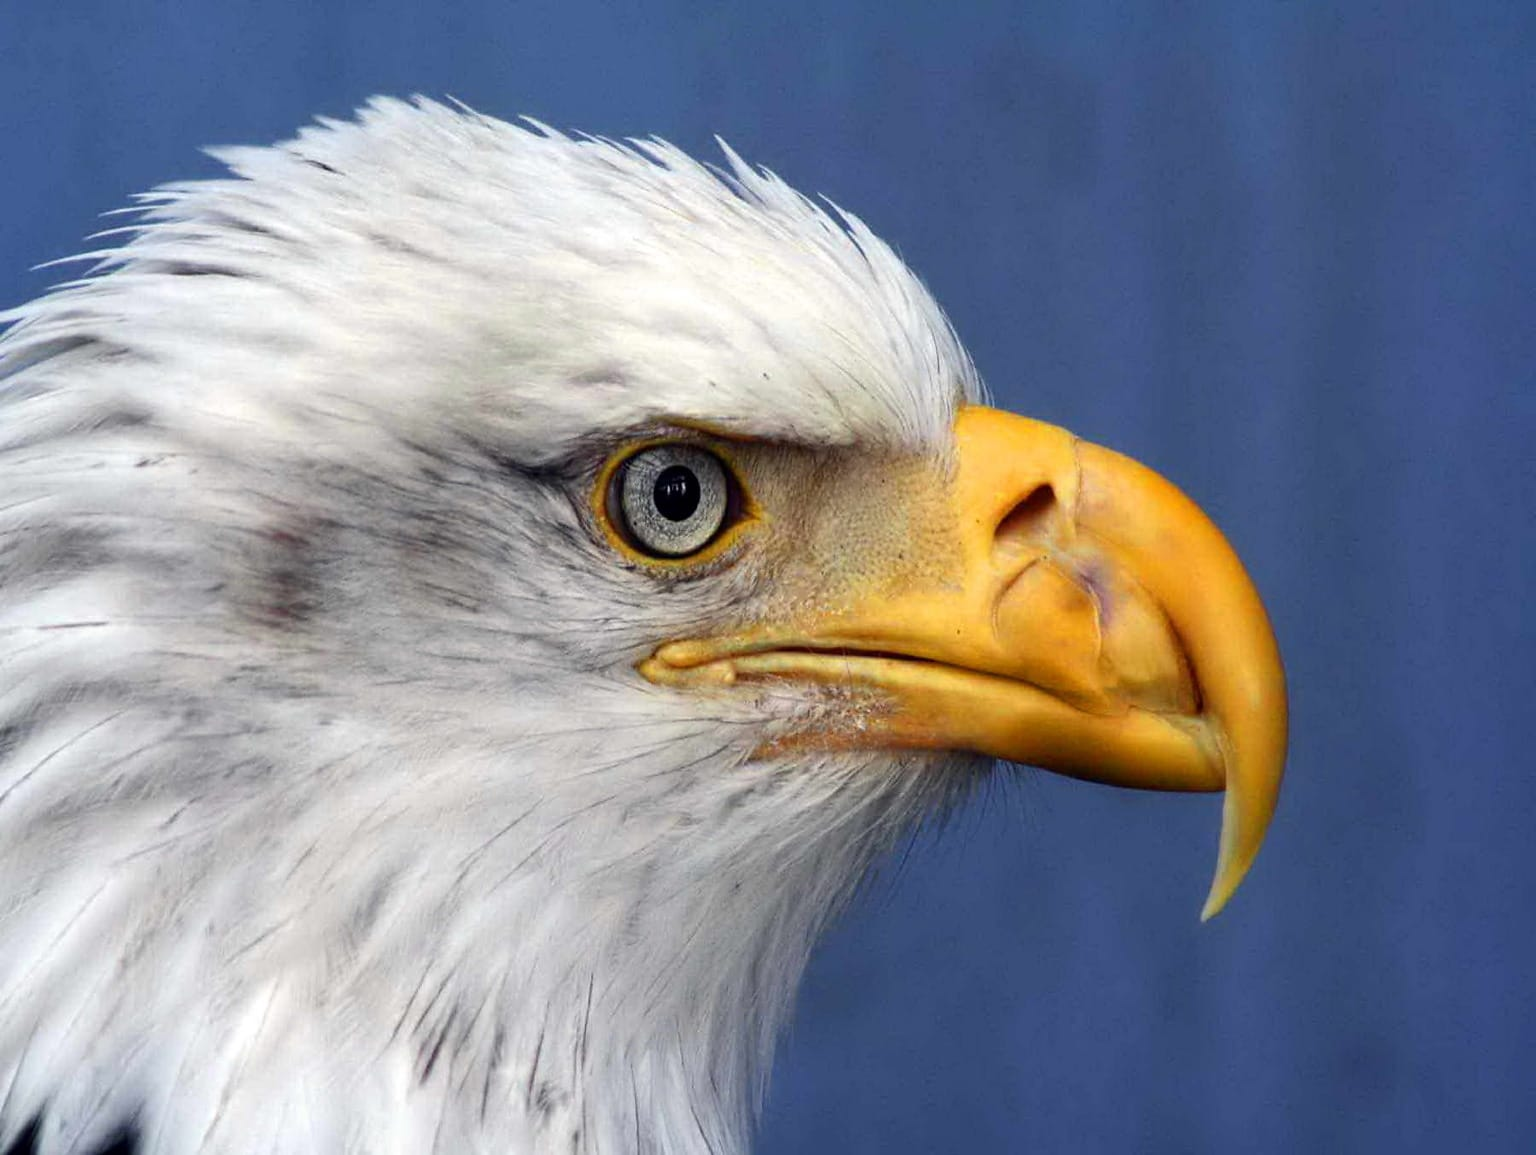
\includegraphics[width=\linewidth]{../data/images/Eagle.jpg}
    \caption{Original}
  \end{subfigure}\hfill
  \begin{subfigure}{0.32\textwidth}
    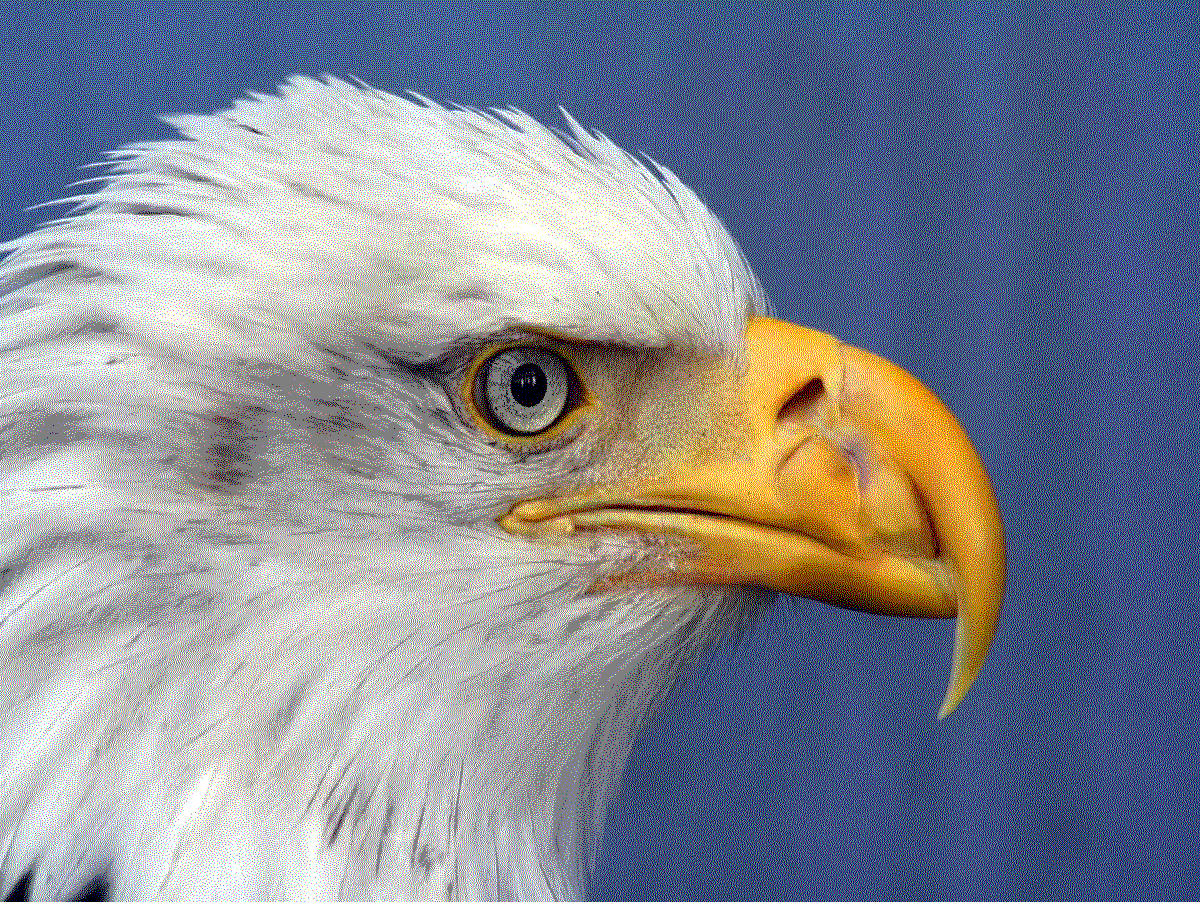
\includegraphics[width=\linewidth]{../output/Section_5_2/Figure_5_2.png}
    \caption{Floyd-Steinberg}
  \end{subfigure}
  \begin{subfigure}{0.32\textwidth}
    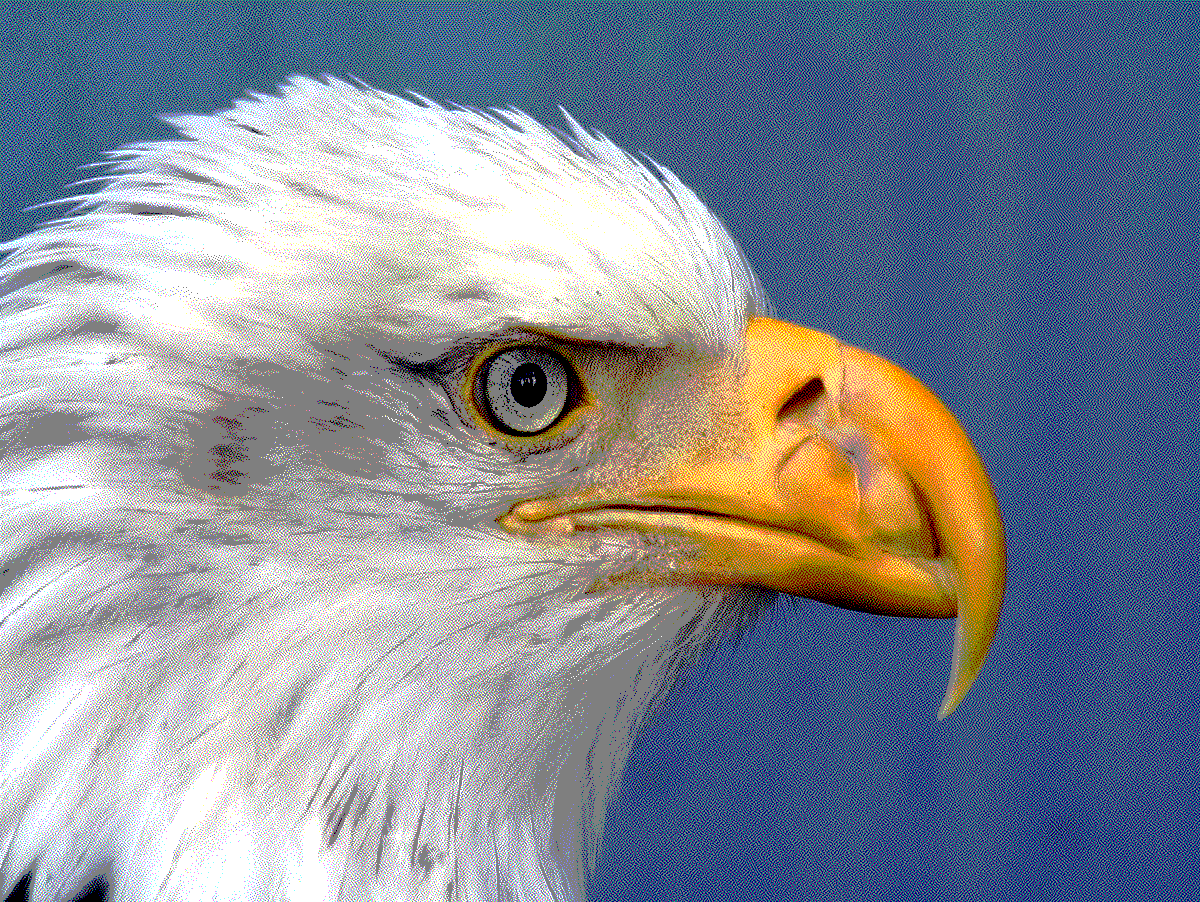
\includegraphics[width=\linewidth]{../output/Section_5_2/Figure_5_3.png}
    \caption{Atkinson}
  \end{subfigure}
  \begin{subfigure}{0.32\textwidth}
    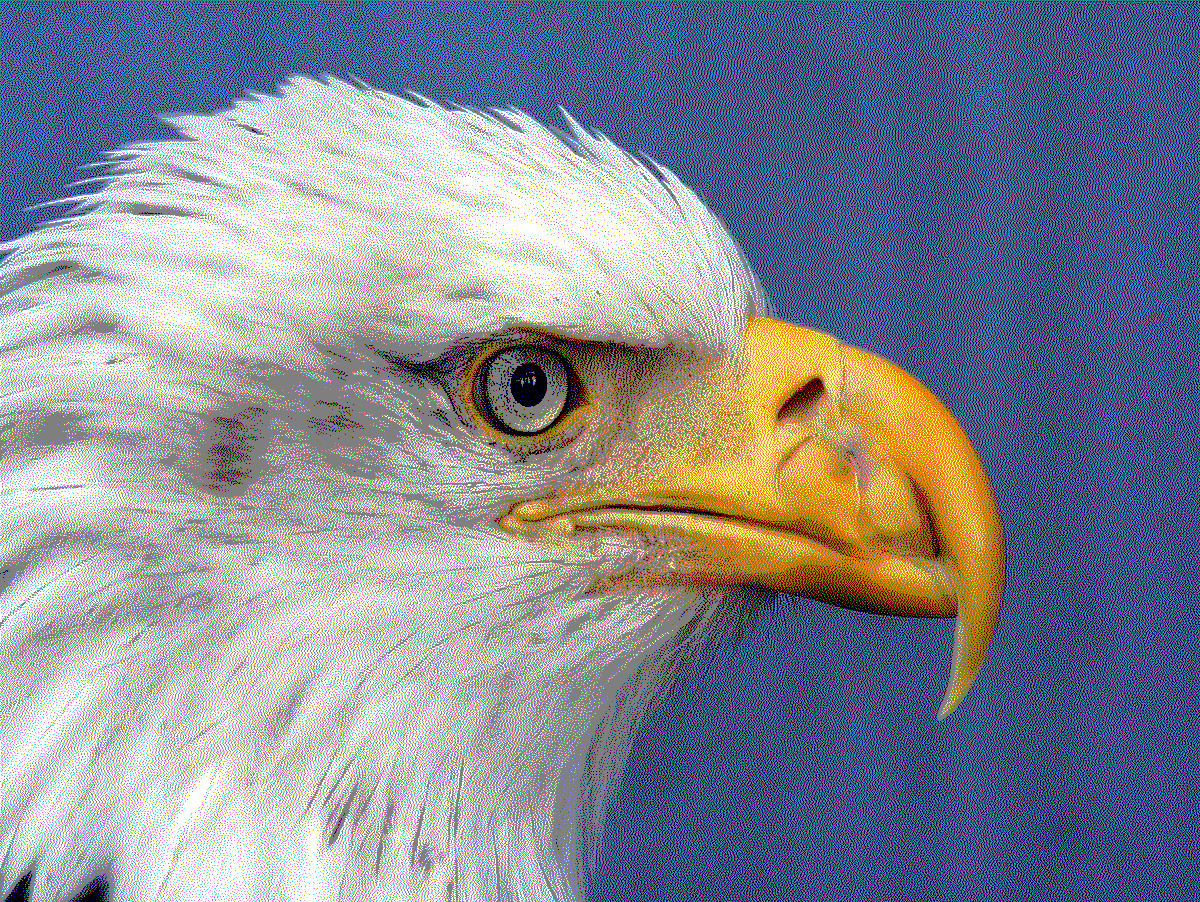
\includegraphics[width=\linewidth]{../output/Section_5_2/Figure_5_4.png}
    \caption{Jarvis--Judice--Ninke}
  \end{subfigure}
  \begin{subfigure}{0.32\textwidth}
    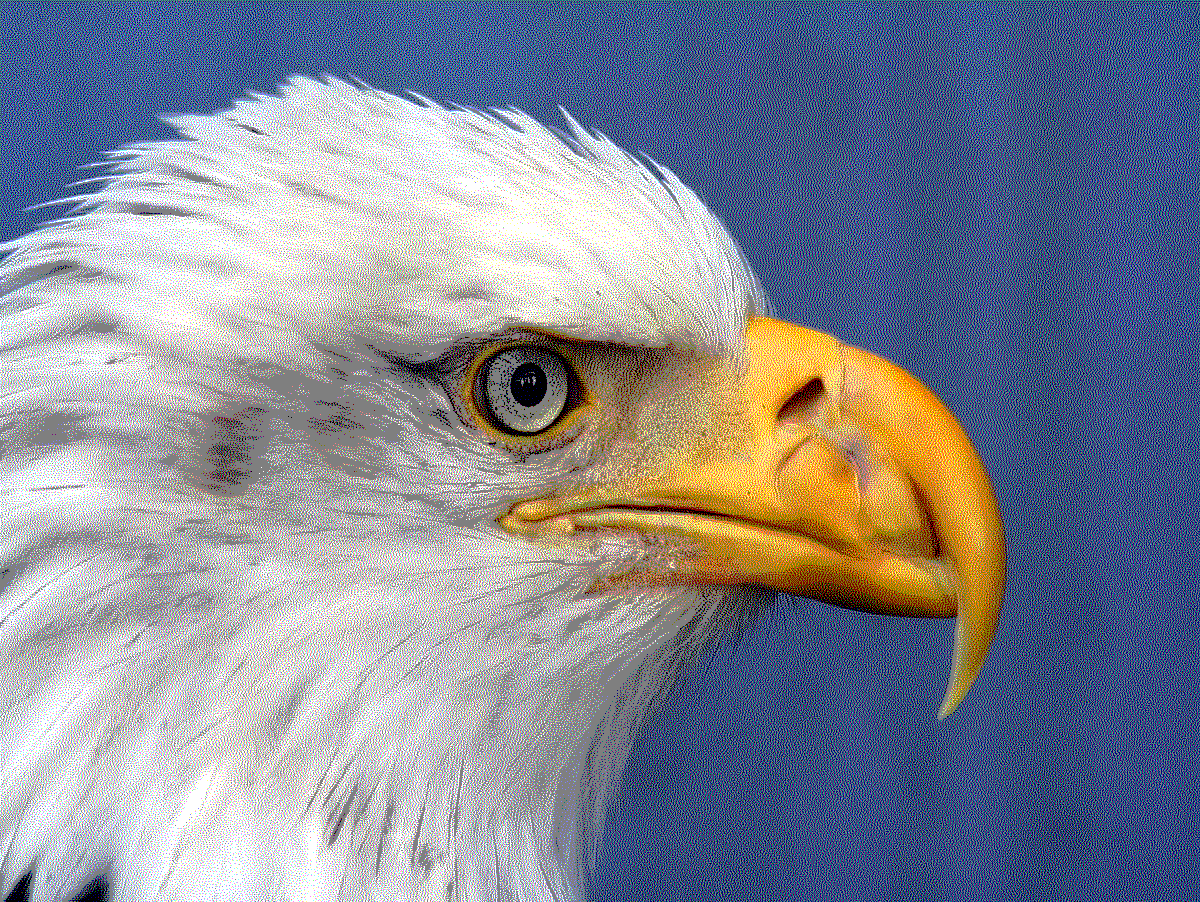
\includegraphics[width=\linewidth]{../output/Section_5_2/Figure_5_5.png}
    \caption{Sierra}
  \end{subfigure}
  \caption{Different Dithering Algorithms applied to the same image.}
\end{figure}

All four algorithms below are \emph{error-diffusion} methods. Pixels are
processed in scan order. For the current pixel at $(x,y)$:
\begin{align}
  \text{old} &= I(x,y), \qquad \text{new} = q(\text{old}), \qquad
  e = \text{old} - \text{new}, \\
  I(x+d_x,\,y+d_y) &\mathrel{+}= \frac{w}{D}\, e
  \quad \text{for each } (d_x,d_y,w) \text{ in the kernel.}
\end{align}
The kernel lists which not-yet-processed neighbours receive a share of the
error, with integer weights $w$ and a divisor $D$. In the matrices below,
$\ast$ marks the current pixel and $\cdot$ marks pixels that are never
modified.

Our implementation uses \emph{serpentine} scanning: the scan direction
alternates every row (and the kernel is mirrored accordingly), which avoids
the diagonal ``worm'' artefacts of always scanning left to right.

\subsubsection{Floyd--Steinberg}
\label{sec:fs}

Published by Floyd and Steinberg in 1976, this is the most widely used
algorithm. It spreads the full error over four neighbours:
\begin{equation}
  \frac{1}{16}
  \begin{pmatrix}
    \cdot & \ast & 7 \\
    3 & 5 & 1
  \end{pmatrix}
\end{equation}

\subsubsection{Atkinson}
\label{sec:atkinson}

Developed by Bill Atkinson at Apple for the original Macintosh, this kernel
spreads the error over six neighbours but divides by 8, so only
$6/8 = 75\%$ of the error is propagated:
\begin{equation}
  \frac{1}{8}
  \begin{pmatrix}
    \cdot & \ast & 1 & 1 \\
    1 & 1 & 1 & \cdot \\
    \cdot & 1 & \cdot & \cdot
  \end{pmatrix}
\end{equation}
Discarding a quarter of the error gives higher contrast: highlights and
shadows tend to saturate to pure white and black, while mid-tones keep
crisp, less noisy detail.

\subsubsection{Jarvis--Judice--Ninke}
\label{sec:jarvis}

This kernel spreads the error over twelve neighbours across three rows:
\begin{equation}
  \frac{1}{48}
  \begin{pmatrix}
    \cdot & \cdot & \ast & 7 & 5 \\
    3 & 5 & 7 & 5 & 3 \\
    1 & 3 & 5 & 3 & 1
  \end{pmatrix}
\end{equation}
The wider spread produces smoother results with finer texture, at the cost of
more computation per pixel.

\subsubsection{Sierra}
\label{sec:sierra}

The three-row Sierra kernel is a lighter relative of Jarvis--Judice--Ninke,
using ten neighbours and a power-of-two divisor:
\begin{equation}
  \frac{1}{32}
  \begin{pmatrix}
    \cdot & \cdot & \ast & 5 & 3 \\
    2 & 4 & 5 & 4 & 2 \\
    \cdot & 2 & 3 & 2 & \cdot
  \end{pmatrix}
\end{equation}

\subsection{Comparison between algorithms}

\begin{table}[htbp]
  \centering
  \caption{Summary of the error-diffusion kernels used.}
  \label{tab:kernels}
  \begin{tabular}{lrrr}
    \toprule
    Algorithm & Neighbours & Divisor $D$ & Error propagated \\
    \midrule
    Floyd--Steinberg        & 4  & 16 & 100\% \\
    Atkinson                & 6  & 8  & 75\%  \\
    Jarvis--Judice--Ninke   & 12 & 48 & 100\% \\
    Sierra                  & 10 & 32 & 100\% \\
    \bottomrule
  \end{tabular}
\end{table}

\todo{Verify publication years and add references for each algorithm.}
\todo{Add side-by-side result figures for the same source image.}

% ------------------------------------------------------------------
\section{Conclusion}
\label{sec:conclusion}

\todo{Summarise your findings. Observations from the analysis tool that may
be worth confirming on real images: (1) a dithered image's histogram collapses
onto $L$ values per channel, yet it still looks smooth because the tone is
carried by the \emph{density} of the dots; (2) error diffusion preserves the
mean brightness almost exactly; (3) pixelising before dithering makes the
pattern visible and keeps computation fast.}

\newpage

% ------------------------------------------------------------------
\addcontentsline{toc}{section}{References}
\begin{thebibliography}{9}

\bibitem{wiki-quant}
Wikipedia contributors.
\emph{Quantization (signal processing)}.
\url{https://en.wikipedia.org/wiki/Quantization_(signal_processing)}.
Accessed \today.

\bibitem{wiki-dither}
Wikipedia contributors.
\emph{Dither}.
\url{https://en.wikipedia.org/wiki/Dither}.
Accessed \today.

\bibitem{wiki-cga}
Wikipedia contributors.
\emph{Color Graphics Adapter}.
\url{https://en.wikipedia.org/wiki/Color_Graphics_Adapter}.
Accessed \today.

\end{thebibliography}

\newpage

% ------------------------------------------------------------------
\appendix
\section{Dithered Image Gallery}
\label{app:gallery}

\begin{table}[htbp]
  \centering
  \caption{Summary of all example images used.}
  \label{tab:images}
  \begin{tabular}{|c|c|c|c|c|c|c|c|}
    \hline 
    Source & Size & Colours & Gray lvls &Mean & Std & Min & Max \\
    \hline
    Apple.png                & 2040x2245  & 538,569 & 249 & 156.37 & 85.12 & 7 & 255 \\
    Banana.jpg               & 3300x3300  & 58,356  & 255 & 246.24 & 19.66 & 1 & 255 \\
    Blackwhite-Wallpaper.jpg & 1920x1080  & 256     & 256 & 113.16 & 111.32 & 0 & 255 \\
    Bruno-Mars.jpg           & 916x639    & 124,696 & 255 & 73.26  & 72.85  & 1 & 255 \\
    Canelo.jpg               & 451x680    & 36,513  & 244 & 73.80  & 55.71  & 0 & 246 \\
    Cat.jpg                  & 554x554    & 90,238  & 246 & 118.83 & 57.10  & 0 & 251 \\
    Chun-Li.png              & 820x523    & 73,098  & 256 & 191.30 & 89.01  & 0 & 255 \\
    Eagle.jpg                & 1536x1155  & 138,380 & 256 & 136.80 & 60.89  & 0 & 255 \\
    Emoji.png                & 1024x1024  & 38,921  & 215 & 197.30 & 54.31  & 41 & 255 \\
    Flowers.jpg              & 1920x1200  & 207,874 & 243 & 109.21 & 61.14  & 0 & 243 \\
    GitHub.jpg               & 474x484    & 506     & 256 & 212.56 & 79.19  & 0 & 255 \\
    Golden-Retriever.jpeg    & 500x500    & 94,919  & 256 & 118.76 & 37.86  & 0 & 255 \\
    Greek-Statue.png         & 1024x1024  & 53,965  & 255 & 63.58  & 59.70  & 0 & 254 \\
    Iron-Man.jpg             & 840x930    & 46,620  & 256 & 220.40 & 63.64  & 0 & 255 \\
    KFC-Logo.png             & 1219x914   & 14,477  & 236 & 152.23 & 92.63  & 20 & 255 \\
    Lanterns.jpg             & 2160x1080  & 76,346  & 256 & 101.17 & 57.59  & 0 & 255 \\
    Mario.jpg                & 1350x1080  & 206,464 & 256 & 195.13 & 79.48  & 0 & 255 \\
    Mona-Lisa.jpg            & 1057x1600  & 272,610 & 256 & 60.15  & 64.78  & 0 & 255 \\
    Parade.jpg               & 1500x1000  & 527,062 & 256 & 139.82 & 63.42  & 0 & 255 \\
    Pen.jpg                  & 1000x1000  & 30,819  & 256 & 240.88 & 46.05  & 0 & 255 \\
    Pokémon-Legends-ZA.jpg   & 1424x800   & 158,072 & 256 & 75.48  & 45.46  & 0 & 255 \\
    Rock.png                 & 1280x960   & 166,146 & 231 & 181.19 & 63.13  & 25 & 255 \\
    Samus.png                & 1529x1034  & 159,799 & 256 & 214.27 & 74.93  & 0 & 255 \\
    Sonic.png                & 1209x1677  & 16      & 15  & 183.07 &  92.06 & 0 & 255 \\
    Sphere.jpg               & 630x630    & 23,319  & 210 & 143.77 & 70.64  & 44 & 255 \\
    Starry-Night.jpg         & 565x353    & 133,414 & 256 & 110.87 & 66.03  & 0 & 255 \\
    Tennis-Balls.jpg         & 1600x900   & 71,200  & 235 & 182.29 & 36.45  & 1 & 236 \\
    WiFi.jpg                 & 474x484    & 10,549  & 213 & 194.27 & 80.25  & 42 & 255 \\
    Windows-XP-wallpaper-4K.jpg & 2560x1707 & 125,061 & 219 & 128.74 & 42.59  & 21 & 239 \\
    Yahoo.png                & 920x920    & 26,412  & 213 & 107.70 & 79.71  & 43 & 255 \\
    \hline
  \end{tabular}
\end{table}

\IfFileExists{appendix_gallery.tex}{\input{appendix_gallery.tex}}{%
  \todo{Run \texttt{generate\_gallery.py} to create \texttt{appendix\_gallery.tex}.}}

\end{document}